\documentclass[10pt,a4paper]{article}
\usepackage[T1]{fontenc}\usepackage[utf8]{inputenc}
\usepackage{mathpazo,amsmath,amssymb,booktabs,tabularx,array,longtable,graphicx,enumitem}
\usepackage[margin=2.05cm,headheight=13pt]{geometry}
\usepackage{microtype,fancyhdr,lastpage,caption,placeins,hyperref}
\ifdefined\pdfminorversion\pdfminorversion=7\fi
\hypersetup{hidelinks,pdftitle={Supplementary Material: Physics--Semantic RF Event Association}}
\linespread{1.10}\setlength{\parindent}{1.3em}\setlength{\parskip}{2pt}
\newcolumntype{Y}{>{\raggedright\arraybackslash}X}
\renewcommand{\thesection}{S\arabic{section}}
\renewcommand{\thesubsection}{\thesection.\arabic{subsection}}
\renewcommand{\thetable}{S\arabic{table}}\renewcommand{\thefigure}{S\arabic{figure}}
\renewcommand{\theequation}{S\arabic{equation}}
\captionsetup{font=small,labelfont=bf,labelsep=period}
\pagestyle{fancy}\fancyhf{}
\fancyhead[L]{\small Physics--Semantic RF Alignment: Supplementary Material}
\fancyhead[R]{\small\thepage\ of \pageref*{LastPage}}
\fancyfoot[L]{\small Controlled descriptors and public-recording evaluation.}
\newcommand{\ind}{\mathbf{1}}\newcommand{\R}{\mathbb R}
\begin{document}
\begin{center}
{\Large\bfseries Supplementary Material}\par\vspace{5pt}
{\large Physics--Semantic Consistency-Constrained Association of Heterogeneous RF Observations for Multi-Receiver Communication Signal Monitoring}
\end{center}
\noindent This supplement gives implementation details and additional diagnostics for the main manuscript. The executable specification is \texttt{code/experiment.py}. Controlled results use the supplied generated descriptors. Section S7 describes the executed public-recording benchmark and the limits of its packet reference.

\section{Complete nominal generator and observable schema}
\subsection{Generation order and distributions}
Each scene uses \texttt{numpy.random.default\_rng(scene\_seed)}. The receiver ring has radius 2000 m and a scene-wide rotation drawn uniformly from $[0,2\pi)$. For zero-based receiver $s$, the angle is $2\pi s/S$ plus that rotation. Independent scene-shared clock and oscillator residuals are drawn before event parameters, with standard deviations $0.8\,\mu$s and 250 Hz, respectively.

For each of $E=14$ events, emission time is uniform in $[0,120\,\mu\mathrm{s}]$ and carrier is $100\,\mathrm{MHz}+1800m$ Hz plus Gaussian deviation of standard deviation 180 Hz, where $m$ is uniform over $\{0,\ldots,5\}$. Event bandwidth is uniform in $[20,60]$ kHz, duration in $[20,80]\,\mu$s, location in $[-1500,1500]^2$ m, and protocol over four classes. Generation then visits events $e=1,\ldots,E-1$. With probability 0.25, it selects an earlier event uniformly and copies its time, carrier, bandwidth, and duration, adding independent Gaussian perturbations of standard deviations $1.5\,\mu$s, 150 Hz, 2 kHz, and $2\,\mu$s. Copied bandwidth and duration are floored at 1 kHz and $1\,\mu$s. Location and protocol are not copied. Earlier events may themselves be copies; resulting emission times are not clipped back to the initial window.

\paragraph{Interpretation of the parameters.}
The 14 events are 14 transmission instances, indexed 0--13, rather than 14 classes or receiver reports. The four class labels are anonymous $Q_1$--$Q_4$ and have no assigned protocol names. The 1800 Hz value is carrier-center spacing; 20--60 kHz is the initial bandwidth range. Their overlap is intentional and does not establish that a real detector can resolve the transmissions. The 180 Hz standard deviation describes the event carrier perturbation before collision overrides, not a Gaussian signal spectrum, receiver noise power, or bandwidth. An event's common carrier cancels in a same-event frequency difference; the receiver residuals and measurement errors do not. The collision override can move bandwidth outside its initial range. A generated start time is not an observation-window truncation rule for the whole burst.

\texttt{results/event\_ledger\_r00\_test000.csv} gives all 14 event instances for seed 1020000, including their final parameters, anonymous classes, collision parents, detected receivers, and report counts. Its 43 genuine reports and two clutter reports reproduce the delivered first test scene. \texttt{code/audit\_event\_definitions.py} checks that reproduction without modifying or refitting the original experiment.

Receivers are visited in index order. Each detects an event with probability 0.8, and independently produces a Poisson number of clutter reports with mean 0.8. Clutter draws its own time, channel, bandwidth, duration, and protocol from the corresponding basic ranges, uses zero propagation delay, and receives a unique singleton truth label. Non-clutter propagation delay is distance divided by $c=299{,}792{,}458$ m/s. Both report types include the receiver's shared residual and independently drawn detector noise.

Receiver $s\in\{0,\ldots,S-1\}$ has timing, carrier, bandwidth, and duration measurement standard deviations $(0.6+0.4s)\,\mu$s, $(120+80s)$ Hz, $(1500+300s)$ Hz, and $(1+0.3s)\,\mu$s. Timing noise is nominally Gaussian. The same receiver's residual bias is reused for its reports; it is not resampled for each pair. Observed bandwidth and duration are floored at 1 Hz and $10^{-9}$ s. These small positivity floors apply to the generated descriptors and are distinct from the collision-parameter floors above.

Missing semantics are selected with probability 0.10 and wrong labels with probability 0.12. A wrong label is obtained by adding a uniformly selected nonzero class offset modulo four. Confidence is uniform on $[0.45,0.90]$ when wrong and $[0.60,0.95]$ otherwise; the remaining probability is equally split among the other classes. Missingness replaces the whole vector by $(1/4,1/4,1/4,1/4)$. Native column $a$ at receiver $s$ denotes canonical class $(a+s)\bmod4$ in zero-based code indexing. Frequency unit is independently selected from Hz, kHz, and MHz. Finally, all observations and their evaluation labels are shuffled by the same permutation. The executable preserves this exact random-number draw order.

\subsection{Saved data and inference boundary}
The nominal data are stored in thirty compressed CSV files, covering ten replications and three splits. Each row represents one report. Table~\ref{tab:schema} separates admissible inference inputs from administrative and evaluation columns. True source positions are absent from the observation tables; receiver positions are available as sensor metadata.
\begin{table}[!htb]\caption{Observation CSV schema, grouped by purpose.}\label{tab:schema}
\small\renewcommand{\arraystretch}{1.12}
\begin{tabularx}{\linewidth}{@{}p{5.7cm}Y@{}}\toprule
Field or group & Meaning and use \\\midrule
\texttt{receiver}, \texttt{receiver\_x\_m}, \texttt{receiver\_y\_m} & Receiver identity and known planar position; inference input. \\
\texttt{time\_s}, \texttt{frequency\_value}, \texttt{frequency\_unit} & Time and native carrier encoding. Unit code 0/1/2 means Hz/kHz/MHz. \\
\texttt{bandwidth\_hz}, \texttt{duration\_s} & Positive observed bandwidth and duration. \\
\texttt{sigma\_time\_s}, \texttt{sigma\_frequency\_hz}, \texttt{sigma\_bandwidth\_hz}, \texttt{sigma\_duration\_s} & Declared per-observation measurement standard deviations. \\
\texttt{declared\_clock\_s}, \texttt{declared\_freq\_bias\_hz} & Declared scene-shared receiver residual standard deviations. They are not realized bias corrections. \\
\texttt{native\_semantic\_0} through \texttt{native\_semantic\_3} & Native probability vector, requiring the known receiver permutation. \\
\texttt{truth\_event}, \texttt{is\_clutter} & Generation/evaluation labels; never used to construct features or gates. \\
\texttt{replicate}, \texttt{split}, \texttt{scene}, \texttt{scene\_seed} & Audit and data-selection metadata; never scorer inputs. \\\bottomrule
\end{tabularx}\end{table}

\section{Stress overrides, scorer settings, and split schedule}
\subsection{Controlled shifts}
All stress conditions change the generator while freezing nominally fitted scalers, model parameters, temperatures, and gate multiplier $k=3.5$. Table~\ref{tab:overrides} specifies the twelve named scenarios. A matched uncertainty declaration is changed only where explicitly stated; physical measurement-noise standard deviations retain their nominal formulas.
\begin{table}[!htb]\caption{Exact overrides for named stress conditions. Unlisted settings retain their nominal values.}\label{tab:overrides}
\small\renewcommand{\arraystretch}{1.12}
\begin{tabularx}{\linewidth}{@{}p{4.4cm}Y@{}}\toprule
Condition & Override \\\midrule
Nominal stress reference & No override; separate stress scene seeds. \\
Dense events & $E=28$. \\
Missed detections & Per-event, per-receiver detection probability 0.55. \\
Clutter & Poisson clutter mean 2.5 per receiver. \\
Semantic error & Wrong-class probability 0.45. \\
Missing semantics & Uniform-vector probability 0.65. \\
Clock misspecification & Actual shared clock s.d. $6\,\mu$s; declaration remains $0.8\,\mu$s. \\
Oscillator misspecification & Actual shared frequency-bias s.d. 1.5 kHz; declaration remains 0.25 kHz. \\
Positive delays & Independently, 20\% of reports add an exponential timing delay with mean $8\,\mu$s. This is a descriptor contamination, not multipath waveform simulation. \\
Heavy-tailed timing & Replace standard Gaussian timing jitter by $t_3/\sqrt3$, preserving finite variance. \\
Unseen receiver count & $S=5$; use the same ring construction, error formulas, and known native-class permutation. \\
Confidently wrong receiver & At $s=S-1$, force class $(q+1)\bmod4$ with confidence 0.99 and no missing semantic vector. \\\bottomrule
\end{tabularx}\end{table}

The semantic sweep uses wrong-label probabilities $0,0.1,0.25,0.4,0.6,0.75$. The clock sweep uses actual standard deviations $0,0.8,2,5,10,20\,\mu$s, each with either fixed declaration $0.8\,\mu$s or a matched declaration. The scaling sweep uses event counts 8, 16, 32, and 64. Together these make $12+6+12+4=34$ settings. Each uses 20 scenes per replication, with seed $10^6+10^5r+30{,}000+k$. Reusing this schedule couples draws across settings where their control flows allow it; these settings are not statistically independent datasets.

The gate-width sweep uses $k\in\{1,2,3,3.5,5\}$ and the first 20 nominal test scenes of each replication. The small exact audit uses six additional seeds per replication, $10^6+10^5r+50{,}000+k$, with $E=4$, clutter mean 0.3, collision probability 0.5, and initial time window $35\,\mu$s. It yields 60 instances of 11--19 observations. All nominal, stress, and exact seed families are disjoint, except for the deliberate reuse of the same stress seeds across interventions.

\subsection{Feature selection, fitting, and decoding variants}
The physical feature order is absolute normalized timing difference, excess normalized timing difference, normalized carrier difference, normalized bandwidth difference, and normalized duration difference, each transformed by $\log(1+x)$. Weighted semantic compatibility is feature six. Timing-only fitting selects features 1--2, carrier-only selects feature 3, semantics-only selects feature 6, and physical-only selects features 1--5. Joint, raw-frequency, and unweighted variants use six features, with only the stated input changed.

Linear variants use \texttt{StandardScaler} followed by \texttt{LogisticRegression(C=1,max\_iter=500)} with the library's default unbalanced binary log loss, unpenalized intercept, and L-BFGS solver. Means and population standard deviations are fitted on all cross-receiver training pairs. The histogram-gradient-boosted comparator uses 100 iterations, 15 maximum leaf nodes, learning rate 0.08, $L_2$ regularization 1, random state 123, and disabled early stopping. It consumes unstandardized features; its logit is computed from clipped predicted probabilities. No hyperparameter search uses test data.

Every scorer fits a scalar temperature by bounded minimization in $\log T\in[\log0.1,\log10]$, using admitted calibration pairs and numerical tolerance $10^{-7}$. Only named calibrated variants apply it. The decoder uses pre-gate probabilities clipped to $[10^{-12},1-10^{-12}]$ before obtaining signed weights. The gate determines feasibility independently of this clipping. Dense gain arrays are scanned in deterministic index order and merged only above $10^{-10}$.

The assignment baseline forms an optional bipartite assignment for each unordered receiver pair. Dummy columns have zero gain, gate-rejected entries have numerical gain $-10^6$, and only real assignments with positive gain are united. Local one-to-one assignments may still conflict after union. The no-receiver-exclusivity ablation gives same-receiver edges neutral, unscored weights. The no-complete-gate ablation omits all-pair gate feasibility but keeps receiver exclusivity. Other objective components are unchanged in both ablations.

\section{Metric definitions and statistical denominators}
\subsection{Pair metrics and reliability bins}
For $n$ cross-receiver pairs, let $y_a\in\{0,1\}$ and $p_a\in[0,1]$ denote truth and reported probability. The reported probability includes gate-forced zeros. With $\epsilon=10^{-12}$ and $\widetilde p_a=\min(1-\epsilon,\max(\epsilon,p_a))$,
\begin{align}
 \operatorname{Brier}&=n^{-1}\sum_{a=1}^{n}(p_a-y_a)^2,\\
 \operatorname{NLL}&=-n^{-1}\sum_{a=1}^{n}\big[y_a\log\widetilde p_a+(1-y_a)\log(1-\widetilde p_a)\big].
\end{align}
AUROC and non-interpolated AP are computed by scikit-learn on the same set. ECE divides $[0,1]$ into ten equal-width bins, including $p=1$ in the last bin, and evaluates
\begin{equation}
 \operatorname{ECE}=\sum_{b:|B_b|>0}\frac{|B_b|}{n}
 \left|\frac{1}{|B_b|}\sum_{a\in B_b}p_a-
 \frac{1}{|B_b|}\sum_{a\in B_b}y_a\right|.
\end{equation}
Saved pair tables include both all-pair ECE and ECE conditioned on admission. Empty bins contribute nothing. Rejection produces many exact zero scores, so an all-pair summary can hide confidence errors among the admitted candidates.

\subsection{Complete-partition metrics}
Let $C(i)$ and $G(i)$ denote the predicted and true clusters containing observation $i$. All unordered observation pairs, including same-receiver pairs, are used for event-pair precision, recall, and F1. Precision or recall with a zero denominator is set to zero; F1 is set to one when both truth and prediction contain no positive pair. These conventions keep empty-positive scenes in the evaluation.

The $B^3$ measures are
\begin{equation}
 P_{B^3}=\frac1N\sum_i\frac{|C(i)\cap G(i)|}{|C(i)|},\qquad
 R_{B^3}=\frac1N\sum_i\frac{|C(i)\cap G(i)|}{|G(i)|},\qquad
 F_{B^3}=\frac{2P_{B^3}R_{B^3}}{P_{B^3}+R_{B^3}}.
\end{equation}
For contingency counts $n_{uv}=|C_u\cap G_v|$, row totals $n_{u\cdot}$, column totals $n_{\cdot v}$, and $M=\binom N2$, ARI uses
\begin{equation}
 \operatorname{ARI}=\frac{A-BC/M}{(B+C)/2-BC/M},\quad
 A=\sum_{u,v}\binom{n_{uv}}2,\quad B=\sum_u\binom{n_{u\cdot}}2,\quad C=\sum_v\binom{n_{\cdot v}}2.
\end{equation}
Degenerate partitions follow scikit-learn's convention. Exact visible-event recovery averages the indicator that each true cluster of size at least two appears unchanged in the predicted partition. It equals one if no such true cluster exists. Completely unobserved events and true singletons are not in its denominator.

Receiver-violation rate is the fraction of predicted non-singleton clusters containing repeated receiver IDs; it is zero if there are no predicted non-singletons. Gate-violation rate is the number of predicted within-cluster, cross-receiver edges that fail the nominal $k=3.5$ gate, divided by all predicted within-cluster cross-receiver edges, or zero for an empty denominator. Clutter attachment is the fraction of clutter observations placed in non-singleton clusters, or zero when no clutter exists. The gate sweep reports only its own gate recall, retained fraction, and F1, avoiding reuse of the nominal gate-violation definition at a different $k$.

\subsection{Aggregation and uncertainty}
Pair metrics pool scenes within each replication. Partition and runtime metrics first average scenes within a replication. For $R=10$ replication estimates $x_r$, the reported interval is $\bar x\pm t_{0.975,9}s/\sqrt{10}$, with $s^2=\sum_r(x_r-\bar x)^2/(R-1)$. A method difference is formed within replication before applying the same calculation. Reused test scenes permit paired comparisons but do not make the millions of pair entries independent trials. The intervals describe repeated simulation and fitting under this generator; they do not account for simulator misspecification. No familywise multiple-comparison correction is claimed.

\section{Additional diagnostic results and optimization checks}
\begin{figure}[!htb]\centering
\begin{minipage}[t]{.49\linewidth}\centering
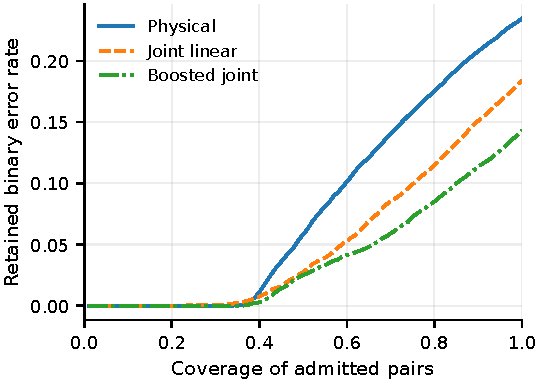
\includegraphics[width=\linewidth]{figures/supp_risk_coverage.pdf}
\caption{Selective admitted-pair risk on held-out replication 0.}
\label{fig:risk}
\end{minipage}\hfill
\begin{minipage}[t]{.49\linewidth}\centering
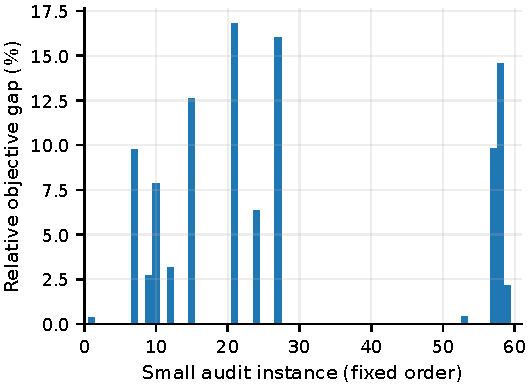
\includegraphics[width=\linewidth]{figures/supp_exact_gap.pdf}
\caption{Greedy objective loss on the 60 exact-audit instances.}
\label{fig:gap}
\end{minipage}
\end{figure}

Figure~\ref{fig:risk} ranks admitted pairs by confidence $\max(p,1-p)$, with stable tie sorting. At each retained fraction it reports the cumulative error of binary decisions at $p\geq0.5$. Coverage is relative to admitted pairs only. This diagnostic does not produce a partial event partition or prove that independently retaining confident pairs preserves global feasibility. Curve points are drawn directly from the stored prediction files, and the exact points are exported as CSV.

Figure~\ref{fig:gap} uses relative objective gap $(J^*-J_g)/\max(|J^*|,10^{-9})$. Forty-seven of 60 cases match the optimum to numerical tolerance $10^{-8}$; the mean gap is 1.71\% and the maximum is 16.82\%. A mixed-integer result is accepted only if SciPy/HiGHS reports success with requested relative gap zero. A 20-second solver limit is imposed per case, and an unproven incumbent raises an error rather than entering the results as exact.

The separate four-node construction has positive edges $w_{12}=5$ and $w_{13}=w_{24}=4$, with $w_{14}=w_{23}=w_{34}=-10$. All receivers are distinct and all gates admit. After merging $\{1,2\}$, gains to nodes 3 and 4 are both $-6$, and edge 3--4 is negative. Greedy inference stops at score 5, while partition $\{1,3\},\{2,4\}$ has score 8. This example demonstrates an irreversible early merge, independently of the RF generator and trained scorer.

\begin{figure}[!htb]\centering
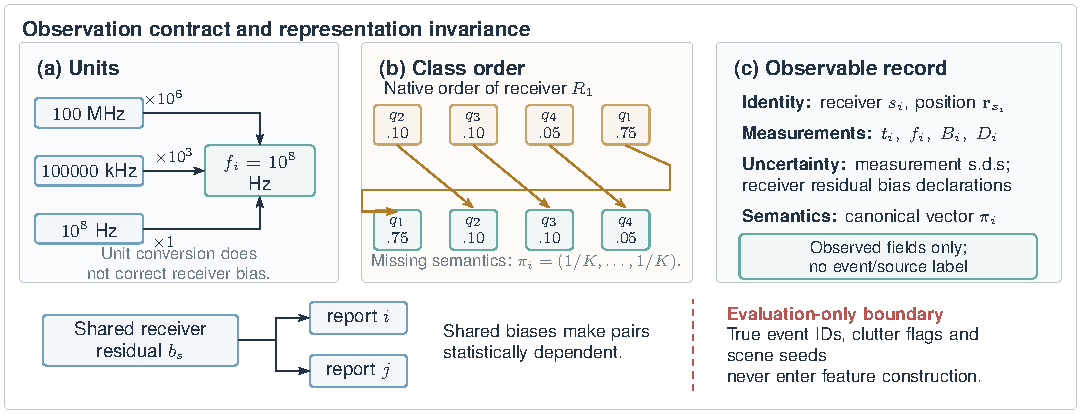
\includegraphics[width=\linewidth]{figures/fig03_contract.pdf}
\caption{Canonical observation interface. (a) Known unit scales recover the same frequency without estimating the receiver's residual bias. (b) A known permutation maps the native order of $R_1$ to the common class order; values are preserved. (c) Inference uses observable record fields. The lower branch distinguishes scene-shared receiver residuals from independent measurement errors, and separates evaluation-only labels from the feature path.}\label{fig:contract}\end{figure}

\begin{figure}[!htb]\centering
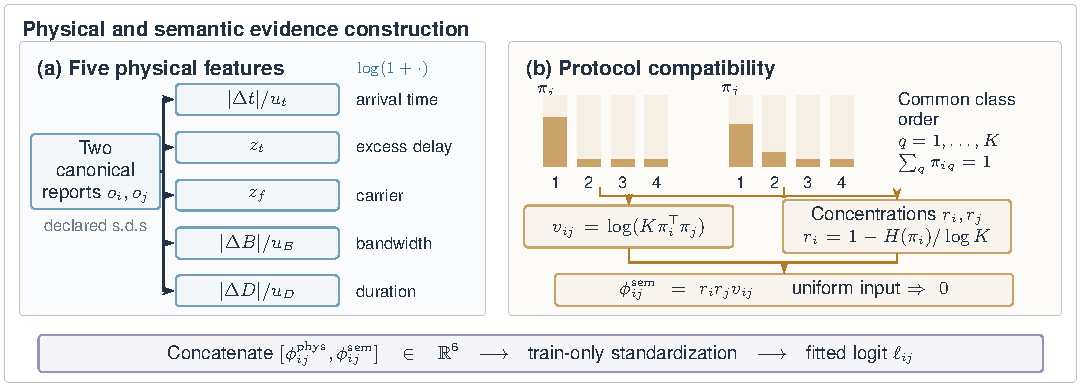
\includegraphics[width=\linewidth]{figures/fig05_evidence.pdf}
\caption{Feature-level decomposition. The physical branch applies $\log(1+\cdot)$ to five uncertainty-normalized residuals. Both canonical protocol distributions feed the dot-product agreement and their respective entropy calculations. The plotted distributions are illustrative vectors $(.7,.1,.1,.1)$ and $(.6,.2,.1,.1)$, not classifier measurements. A uniform distribution contributes zero weighted semantic evidence. The six-dimensional concatenation is standardized using training scenes only.}\label{fig:evidence}\end{figure}

\begin{figure}[!htb]\centering
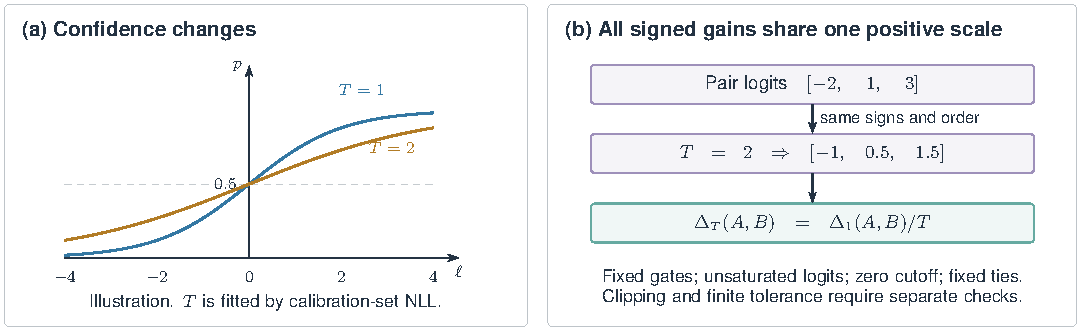
\includegraphics[width=\linewidth]{figures/fig06_temperature.pdf}
\caption{Calibration versus partition decisions. (a) Illustrative sigmoid curves show a confidence change without moving the $0.5$ crossing. (b) Dividing all finite unsaturated logits by a common positive $T$ rescales every signed merge gain by the same factor. Fixed-gate, exact-arithmetic ordering is preserved. The fitted temperatures and empirical probability quality are evaluated separately; this diagram is not a claimed calibration result.}\label{fig:temperature}\end{figure}

\begin{table}[!htb]\caption{Additional controlled partition metrics. Exact denotes full recovery of a visible event; Rx and Gate use the denominators defined in Section S3.}\small\begin{tabularx}{\linewidth}{@{}Yrrrrr@{}}
\toprule
Scoring and decoding & F1 [95\% CI] & ARI & Exact & Rx (\%) & Gate (\%) \\
\midrule
Physical, constrained & 0.6813 [0.6658, 0.6968] & 0.6683 & 0.4072 & 0.00 & 0.000 \\
Boosted, constrained & 0.8238 [0.8181, 0.8295] & 0.8160 & 0.6189 & 0.00 & 0.000 \\
Joint, connected components & 0.6764 [0.6641, 0.6887] & 0.6549 & 0.4909 & 21.14 & 0.725 \\
Pairwise assignment + union & 0.7797 [0.7741, 0.7853] & 0.7671 & 0.5973 & 10.49 & 0.127 \\
Joint, constrained & 0.7798 [0.7713, 0.7883] & 0.7704 & 0.5375 & 0.00 & 0.000 \\
Without receiver exclusivity & 0.7361 [0.7300, 0.7422] & 0.7227 & 0.4736 & 14.33 & 0.000 \\
Without all-pair gate check & 0.7796 [0.7710, 0.7882] & 0.7702 & 0.5375 & 0.00 & 0.073 \\
Unweighted, constrained & 0.7983 [0.7892, 0.8074] & 0.7897 & 0.5652 & 0.00 & 0.000 \\
\bottomrule
\end{tabularx}
\end{table}
\FloatBarrier

\section{Notation and implementation correspondence}
\small\renewcommand{\arraystretch}{1.10}
\begin{longtable}{@{}>{\raggedright\arraybackslash}p{3.0cm}>{\raggedright\arraybackslash}p{2.5cm}>{\raggedright\arraybackslash}p{10.5cm}@{}}
\caption{Mathematical notation used in the main manuscript and supplement.}\label{tab:notation}\\
\toprule Symbol & Unit or type & Definition \\\midrule\endfirsthead
\toprule Symbol & Unit or type & Definition (continued) \\\midrule\endhead
\bottomrule\endfoot
$S,s,s_i$ & Counts/indices & Number of receivers; zero-based receiver index; receiver of report $i$. \\
$E,e$ & Counts/indices & Generated event count and hidden event index. $E$ is not supplied to inference. \\
$N,i,j,\nu$ & Counts/indices & Number of reported observations and observation indices. \\
$K,q,q_e$ & Counts/indices & Number of protocol classes, class index, hidden event class. Math uses classes $1,\ldots,K$; code uses $0,\ldots,K-1$. \\
$\mathbf r_s,\mathbf x_e$ & m, vectors & Known receiver position and hidden event position. \\
$c$ & m/s & Assumed propagation speed, 299,792,458. \\
$\tau_e,t_i$ & s & Hidden emission time and observed arrival time. \\
$f_e,f_i$ & Hz & Hidden event carrier and canonicalized observed carrier. \\
$B_e,B_i$ & Hz & Hidden event bandwidth and observed bandwidth. \\
$D_e,D_i$ & s & Hidden event duration and observed duration. \\
$b_s,d_s$ & s; Hz & Residual receiver clock and oscillator offsets, shared within a scene. The bold vector $\mathbf d$ collects oscillator offsets; path-length labels $d_i$ in the gate diagram are instead distances in metres. \\
$\epsilon_i^t,\epsilon_i^f,\epsilon_i^B,\epsilon_i^D$ & Corresponding units & Independent measurement errors before positivity clipping of bandwidth and duration. \\
$m_i$ & s & Additional nonnegative timing contamination; zero nominally. \\
$\sigma_i^t,\sigma_i^f,\sigma_i^B,\sigma_i^D$ & Corresponding units & Declared measurement-error standard deviations. \\
$\Sigma_b,\Sigma_d$ & s$^2$; Hz$^2$ & Declared receiver-residual covariance matrices; off-diagonal values are zero nominally; the review audit also tests matched correlated clock declarations. \\
$u_{t,ij},u_{f,ij},u_{B,ij},u_{D,ij}$ & s; Hz; Hz; s & Positive declared standard deviations of pair measurement differences. \\
$v_i,u_i,\alpha(u_i)$ & Native value/unit/scale & Native carrier number, native unit, and conversion to hertz. $u_i$ is a unit label, not the pair standard deviation $u_{t,ij}$. \\
$\pi_i,\pi_{iq}$ & Probability vector & Canonical protocol belief and its class-$q$ entry. \\
$\Delta t_{ij},\Delta f_{ij},\Delta B_{ij},\Delta D_{ij}$ & Corresponding units & Signed differences of corresponding observed values. \\
$h_{ij}$ & s & Receiver separation divided by propagation speed. \\
$z_{t,ij},z_{f,ij},k$ & Dimensionless & Excess timing residual, carrier residual, and gate multiplier. \\
$g_{ij},\ind[\cdot]$ & Binary & Gate admission and indicator function. \\
$y_{ij},\Phi$ & Binary; function & True same-event indicator and standard-normal cumulative distribution function. \\
$\phi^{\rm phys},\phi^{\rm sem},\phi,\widetilde\phi$ & Feature vectors/scalar & Five physical features, weighted semantic scalar, six-dimensional concatenation, and standardized feature vector. \\
$v_{ij},H(\pi_i),r_i$ & Dimensionless & Log compatibility, Shannon entropy in natural units, and normalized concentration. Concentration is not correctness. \\
$\epsilon$ & Dimensionless & Numerical probability floor $10^{-12}$, distinct from measurement-error symbols with indices/superscripts. \\
$\mu,\sigma$ & Feature vectors & Training-set means and scales for componentwise standardization; not the measurement-error standard deviations. \\
$\beta_0,\beta,\ell_{ij}$ & Dimensionless & Fitted linear intercept, coefficient vector, and pair logit. \\
$C_{\rm reg}$ & Positive scalar & Inverse regularization setting; equal to one. \\
$\mathcal T,\mathcal V_g$ & Pair sets & All cross-receiver training pairs and admitted calibration pairs. \\
$T,T^*$ & Positive scalar & Temperature and its calibration optimum. \\
$p^{\rm cal}_{ij},\widehat p_{ij}$ & Probability or score & Pre-gate calibrated probability and final gate-masked score. \\
$w_{ij},W,G$ & Weights/matrices & Signed pre-gate pair weight, dense symmetric weight matrix, and dense gate mask. \\
$\mathcal C,C,A,B,M$ & Sets/count & Predicted partition, event cluster/current clusters, and unknown number of predicted clusters. Cluster $B$ is distinct from bandwidth $B_i$. \\
$a_{ij},\mathcal S(A)$ & Binary/set & Predicted co-membership and receiver IDs represented in cluster $A$. \\
$J,J_g,J^*$ & Dimensionless & Partition objective, greedy objective, and proven small-instance optimal objective. \\
$F(A,B),\Delta(A,B)$ & Binary; weight sum & Feasible-merge indicator and sum of all signed cross-cluster weights. \\
$\mathrm{TP},\mathrm{FP},\mathrm{FN}$ & Pair counts & Correct, false, and missed predicted co-memberships. \\
$C(i),G(i)$ & Observation sets & Predicted and true cluster of observation $i$ in metric definitions. \\
$R,r,\bar x,s_x$ & Count, index, or statistic & Number of independent replications, replication index, mean estimate, and sample standard deviation across replications. \\
\end{longtable}
\normalsize

\section{Reproduction, audits, and evidence limits}
From the project directory, install the pinned packages and run \texttt{python code/reproduce.py}. The wrapper regenerates ten complete replications, aggregates results, redraws diagrams and statistical figures, compiles both documents, and runs numerical and document checks. A LaTeX installation with \texttt{pdflatex} and TikZ is required for compilation; descriptor experiments require only Python packages and no GPU. To inspect the delivered outputs without refitting, run \texttt{python code/verify\_results.py} and the invariant/diagram tests described in the README.

The audit regenerates all 2400 nominal scenes and checks the raw CSVs against their seeds. It also verifies train/calibration/test seed separation, 12 pair variants and eight partition variants; recomputes summaries and first-replication linear predictions; and checks that constrained decoders have zero violations. Separate invariant tests cover unit conversion, canonical class renaming, neutral missing semantics, exclusion of truth labels from features, rigid receiver-geometry transformations, temperature invariance in unsaturated tests, and the four-node counterexample. Diagram examples undergo numerical checks as well as layout inspection.

Runtime curves use physical/joint stress-decoder timings. The stored nominal runtime of the unweighted ablation includes its score call inside the timed wrapper and should not be treated as a decoder-only comparison; it is not plotted as one. Absolute timings depend on CPU load and library versions. Full reruns should reproduce scientific metrics within floating-point tolerance, but need not reproduce wall-clock times or byte-identical compressed archives.

The nominal benchmark evaluates controlled descriptors. RF waveform extraction, calibration of measured semantic posteriors, covariance estimation, unknown Doppler, and temporal transmitter tracking remain outside its validation scope. Sections S11--S14 examine map completion, correlation, fragmentation, and optimization under controlled conditions. The fifth-receiver test covers only the receiver family specified by the generator. Field validation requires synchronized ground-truth events, measured errors and correlations, known and unknown vocabulary controls, realistic false detections, and evaluation on disjoint receiver, day, and channel splits.
\section{Executed public LoED protocol and additional records}
\subsection{Input provenance, exclusions, and reference interpretation}
The data come from the publisher's six-file LoED sample, DOI \url{https://doi.org/10.5281/zenodo.4121430}, released under CC BY 4.0. The publisher MD5 is \texttt{7370baddc9b546354c26a71cd38981bc}; the download manifest identifies the original ZIP and metadata. The source paper is DOI \url{https://doi.org/10.1145/3419016.3431491}. This benchmark uses measured reception records. We add no simulated noise, protocol posteriors, receiver positions, or uncertainty declarations.

The full physical-payload bytes are base64-decoded, checked for a minimum header length and unconfirmed-uplink message type, and hashed for reference construction. CRC-invalid records are removed. Exact duplicate rows are removed before excluding every payload group with a repeated gateway or a span greater than 5 s. This conservative rule avoids choosing among repeated reports using reference knowledge. Four observations with identities shared across different splits are removed. The per-file inclusion ledger accounts for raw, CRC-valid, type-valid, duplicate, ambiguous, cross-split, and eligible rows. The large exclusion rate in the 2019 training captures selects a restricted reference population, not all over-the-air emissions.

\begin{table}[!htb]\caption{Public-recording inclusion by capture file. Ambiguous rows belong to repeated-gateway or long-span payload groups. Cross-split payload exclusions are applied afterward.}\small\begin{tabular*}{\linewidth}{@{\extracolsep{\fill}}lrrrrr@{}}\toprule
Capture file date & Raw & Valid uplinks & Exact duplicates & Ambiguous & Eligible \\\midrule
2019-03-03 & 122,208 & 79,501 & 40 & 69,891 & 9,570 \\
2019-04-02 & 108,046 & 68,665 & 16 & 60,095 & 8,554 \\
2020-05-02 & 29,977 & 21,366 & 0 & 41 & 21,323 \\
2020-07-03 & 25,659 & 17,271 & 0 & 19 & 17,252 \\
2020-08-03 & 26,588 & 15,282 & 0 & 27 & 15,254 \\
2020-09-02 & 14,392 & 8,444 & 0 & 20 & 8,423 \\
\bottomrule\end{tabular*}
\end{table}

Identical retained payloads define a logical reference packet under these rules. Different physical retransmissions could still produce the same decoded bytes while being missed by complementary gateways. Thus the reference is not an independently instrumented physical-burst annotation. The 5 s eligibility rule uses identity-group timing but is not the association gate; the latter is fitted solely on calibration data. Identity fields, addresses, counters, ports, and row indices are excluded from all pair features.

\subsection{Fitting and measured-input adaptation}
The three earliest files are training data, 3 July 2020 is calibration, and 3 August and 2 September 2020 are test. No observation pairs are formed before this split. Receiver offsets use only training reference matches: pair medians with at least ten examples define equations $b_s-b_r=\operatorname{median}(t_s-t_r)$, weighted by the square root of their count. A minimum-norm least-squares solution fixes unsupported receivers at zero. The supported gateway pair has 256 training matches, a median difference of 0.999985 s, and corrections $+0.4999925$ and $-0.4999925$ s. These are supervised training corrections, not test-derived synchronization.

Calibration reference residuals give the tolerance $G=\max(1\,\mathrm{ms},Q_{0.99})=3.02517$ ms. The three measured features are the log-normalized corrected time difference, reported-frequency mismatch, and decoded-spreading-factor mismatch. A timing-only model uses the first; a metadata model uses all three. Feature scalers and regularized logistic coefficients use training pairs only. Temperatures are fitted on admitted calibration pairs. The metadata temperature is approximately 0.10844; the timing temperature lies near the allowed lower bound 0.1. No partition gain is attributed to this common rescaling.

The generic decoder is reused with the empirical time gate, not the Gaussian geometry gate. The adapter disables absent gate modalities; it does not provide invented receiver positions or RF measurements. Bandwidth metadata is retained for provenance but is not a fitted-uncertainty feature. RSSI and SNR differences are omitted because equal values are not expected at different receivers. All parameters and the uninformative role of protocol-class evidence are frozen before test.

\subsection{Complete-capture evaluation and reproduction}
Fixed 60 s windows use corrected observation times. No reference identity is used to keep matching packets in one window. Predicted cluster labels are made unique across windows, and TP, FP, and FN are counted over each complete capture, including same-receiver false positives and matching references split by boundaries. Complete-reference recovery requires that all reports of a visible reference are recovered without additions. Receiver violations count invalid non-singleton clusters; gate violations count inadmissible cross-receiver edges inside predicted clusters.

Run \texttt{python code/fetch\_loed.py} and \texttt{python code/loed\_benchmark.py}. The first utility verifies publisher checksums and records provenance; the second reads the verified archive and produces inclusion ledgers, separate observations and references, fixed parameters, predictions, and per-capture/pooled metrics in \texttt{results/loed/}. \texttt{python code/scorer\_decoder\_factorial.py} independently runs the four-scorer, three-decoder comparison on the existing controlled scenes and verifies its constrained results against the released original experiment. No new controlled scenes are introduced for that comparison.

Only two gateways remain in the eligible LoED test data, and the two held-out capture files do not support a deployment-population confidence interval. The real result is a reproducible packet-reference check, not validation of the full six-feature RF uncertainty model or a multi-protocol recognizer. The separate measurement and controlled outcomes should not be averaged into a single score.

\section{Representation and class-semantic alignment audit}
The workflow aligns heterogeneous RF observations and produces instance correspondences. This audit uses supplied source-specific field and class mappings. \texttt{code/semantic\_alignment\_audit.py} reuses all 800 original nominal test scenes, frozen joint-linear parameters, and the constrained decoder to compare mapped vectors, uncorrected native column order, and uniform class evidence. Physical features and the gate remain fixed. The intervention changes inputs at test time and is therefore different from training a physical-only model.

For each scene the audit also changes frequency units and reorders the canonical probabilities by independently drawn receiver-specific permutations. The matching registry inverts those re-encodings before the original feature interface is used. The recovered common vectors and physical features are checked against the originals; deterministic partitions agree in all 800 scenes. No event labels enter the representation adapter. This validates handling of known representations, rather than discovery of unknown meanings.

The saved outputs include 2400 scene-condition metric rows, replication summaries for each condition, paired F1 differences, and per-observation predicted labels before and after matched re-encoding. They are retained in \texttt{results/semantic\_alignment/}. The mapping registry has exactly four shared classes and bijective correspondences. Semantic hierarchy, open-set classes, schema discovery, and real waveform-classifier probability calibration are not established by these results. The independent verifier recomputes event-pair metrics from saved labels and original scene references.
\section{Optional incomplete-registry probe}\label{supp:partial_probe}
\subsection{Preserved baseline and small inference wrapper}
The optional module is implemented in \texttt{code/partial\_mapping\_extension.py}. It retains the original generator, entropy-weighted compatibility, scaler, coefficients, temperatures, physical gate and constrained decoder. Its inputs are observable receiver IDs, native probability vectors or decoded-category indicators, physical pair features and gate residuals. Event references, hidden category maps, payload hashes, and source coordinates are kept separately for benchmark construction and evaluation. Existing figures and tables report baseline results; they are not relabeled as evidence of map learning.

The target source has $F$ unanchored native entries. Candidate maps enumerate the $F!$ unused common-class assignments after anchored rows/values are removed. Given provisional groups, each candidate is scored with the original entropy-weighted log feature and frozen model. In particular, no Hungarian update for a bilinear surrogate is substituted. A physical-only initialization avoids using arbitrary native column indices as common meanings. The sequential map estimate is a complete enumeration for the fixed initial groups. Feedback compares a fresh greedy partition with the preceding feasible partition under the current map, retaining the better one, then enumerates maps again. Strict gains exceed $10^{-10}$; ties retain the preceding state and the cap is ten sweeps. Feasibility is inherited from the original decoder. Adaptation objective ascent is not a semantic-correctness or global-optimality guarantee.

\subsection{Controlled reuse and masked entries}
For repetition $r$, scene seeds remain $R_r=10^6+10^5r$, calibration/adaptation $R_r+10{,}000+j$ ($j=0,\ldots,39$), and test $R_r+20{,}000+j$ ($j=0,\ldots,79$). The adapter first reverses the generator's declared cyclic encoding, then re-encodes receiver 1 with a permutation drawn using seed $9{,}100{,}000+r$, stable across adaptation and test. Other maps are known. The correspondence to common class 0 is disclosed; its native index depends on the hidden codebook. The remaining three entries are evaluated, for 30 withheld entries across ten repetitions. No reference instance labels are passed to the mapping module.

The adaptation descriptors come from calibration scenes whose labels were already used in the historical scalar-temperature fit. Their reuse does not create a new independent calibration/adaptation collection. All fitted parameters remain frozen. Map selection uses only the re-encoded descriptors and provisional groups, and test references never select updates. The public probe uses a later adaptation capture. Both probes are exploratory analyses of previously inspected data.

Mapping accuracy counts only withheld entries, excluding the anchor and all known receivers. Controlled F1 averages the 80 scene scores in each repetition before averaging the ten repetition means. The known-map adapter reproduces all 800 original scene F1 values. Five- and 40-scene adaptation recover all three withheld entries in every repetition, while one-scene adaptation recovers 26/30. Sequential and feedback test results tie. The supplied predictions, maps, traces and summaries also include the five-scene condition omitted from the compact main table.

\subsection{Public code hiding and independent later-capture evaluation}
The original six-file LoED filtering, clock corrections, empirical gate, timing scorer and three-feature metadata scorer are retained. The two active original receiver IDs are 0 and 3; local IDs 0 and 1 only simplify the wrapper. The 3 August 2020 capture supplies 15,254 adaptation reports, while 2 September supplies 8423 test reports. Their reference identities do not overlap. At local receiver 1, native SF7/SF12 column meanings are exchanged and withheld, while SF8--SF11 correspondences are fixed. The reference source retains its known SF7--SF12 vocabulary. There are only two candidate maps. Decoded SFs are categorical metadata, not noisy protocol-recognition posteriors; measured time and frequency values are not perturbed.

Initialization uses the original timing-only model. Map candidates and subsequent association use the original metadata model, whose third feature is SF mismatch. Physical features contain only corrected-time residual and reported-frequency mismatch. Payload references are isolated from mapping and decoding. Both withheld entries are recovered. On the later test capture, the learned map yields TP 511, FP 1 and FN 3, exactly matching the complete-map reference. Under unresolved order the counts are TP 35, FP 2 and FN 479. Both methods return feasible partitions. This two-entry correction establishes a limited measured-input mechanism; it cannot establish unknown protocol semantics, recovery of a completely hidden six-class map, or a general benefit over sequential alignment.

Run \texttt{python code/partial\_mapping\_extension.py} and then the accompanying verification script. Results are under \texttt{results/partial\_mapping\_extension/}. Separate mapping and event metrics, objective traces and observation-level predictions make it possible to distinguish missing-registry recovery from a change in the original classifier or decoder.




\section{Proofs of the main propositions}
\subsection{Conditional physical coverage}
The propagation part of $\Delta t_{ij}$ has magnitude at most $h_{ij}$, so failure of the time gate requires timing-error magnitude above $ku_{t,ij}$, with probability at most $2\Phi(-k)$. A true pair's frequency difference has zero mean and standard deviation $u_{f,ij}$, giving the same tail probability. A union bound gives the main-text bound without requiring independence between the two tests.
\subsection{Temperature invariance}
Sigmoid is strictly increasing, so positive rescaling preserves logit ranking and signs. Each within-cluster score and merge gain is divided by $T$, preserving gain ordering and positivity. Induction then gives the same merge sequence.
\subsection{Greedy feasibility and complexity}
Singletons satisfy both constraints. Suppose two valid clusters pass $F(A,B)$. Their receiver sets are disjoint, and all cross edges pass. Their internal edges remain valid. Induction therefore proves feasibility. The main-text merge gain equals the change in $J$. Every accepted merge reduces the cluster count by one. There are at most $N-1$ scans of a dense $N\times N$ gain array. This requires $O(N^3)$ comparisons. The gain and feasibility arrays use quadratic storage.

\section{Independent map-completion audit}
The new audit uses \texttt{code/review\_mapping.py}. Adaptation seed $80{,}000{,}000+100{,}000r+j$ uses $r=0,\ldots,9$ and $j=0,\ldots,39$. Hidden source permutations use seed $83{,}000{,}000+r$. Anchor selection uses $84{,}000{,}000+100r+s$. Wrong-map interventions use $82{,}000{,}000+10{,}000r+10h+v$. Here $h$ is the wrong-entry budget and $v=0,1,2$. Wrong-entry counts are exact. Their values are generated by bijective permutations rather than independently replacing individual labels.

\subsection{Receiver-pair factorization and cost}
Receiver 0 keeps its known naming reference. Fixed partitions determine the co-grouped cross-receiver edges $\mathcal E_A$. Let $\mathcal E_{st}$ contain edges between receivers $s$ and $t$. These sets partition $\mathcal E_A$. Hence
\[
 J_A(\mathbf M,\mathcal C)=\sum_{s<t}\Psi_{st}(M_s,M_t),\qquad
 \Psi_{st}(M_s,M_t)=\sum_{(i,j)\in\mathcal E_{st}}w_{ij}(M_s,M_t).
\]
An edge score depends only on its endpoints' maps. Entropy is invariant under permutation, while the probability inner product depends on the relative permutation. There are at most $K!$ relative permutations for a receiver pair, so the cache needs at most $K!$ distinct feature-score evaluations per pair. The joint map variables nevertheless remain dependent.

Let $E_A=|\mathcal E_A|$. Let $d_s$ be the candidate count at source $s$. A known map has one candidate. Correct anchors give $d_s=(K-a_s)!$ at an unknown source. Let $P$ count receiver-pair terms. The joint domain has $Q=\prod_{s\in\mathcal U}d_s$ states. A conservative preprocessing bound is
\[
 O\!\left(E_A K K!+K\log K\sum_{s<t}d_s d_t\right).
\]
The first term covers relative-permutation dot products on edges. The second covers inverse-permutation construction and pair-table indexing across candidate-map pairs. The implemented broadcast summation then takes $O(PQ)$ time. Its dense objective array uses $O(Q)$ memory. A conservative bound including pair tables is $O(Q+\sum_{s<t}d_sd_t)$, excluding input records. In a dense network, $P$ can grow as $S(S-1)/2$. Receiver-pair factorization is not an $O(U(K!)^2)$ solution to the full coupled search.

For four classes and three unknown receivers, $Q=13{,}824$. For four classes and six unknown receivers, $Q=191{,}102{,}976$. A float64 objective array alone then needs about 1.42 GiB. For six classes and three unknown receivers, $Q=373{,}248{,}000$. Its array needs about 2.78 GiB. These are arithmetic storage estimates. They are not runtime experiments. The delivered implementation rejects more than one million states before array allocation. Larger domains need approximate search, more anchors, or smaller variable blocks. Their accuracy is not evaluated here.

\subsection{Coordinate coupling and a strict counterexample}
Consider two unknown binary class maps and one known reference map. Let $I$ denote identity. Let $P$ denote a swap. Give each reference pair score 1 for $I$ and 0 for $P$. Give the unknown--unknown pair score 3 for equal maps and 0 otherwise. The joint objectives are
\[
\begin{array}{c|cc}
 & M_2=I & M_2=P\\\hline
 M_1=I & 5 & 1\\
 M_1=P & 1 & 3
\end{array}
\]
At $(P,P)$, either single-source change lowers the score from 3 to 1. Strict coordinate ascent therefore stays there. The joint state $(I,I)$ has score 5. This proves that a coordinate fixed point need not solve the conditional joint map block. The example uses constructed pair scores. It is not an RF accuracy experiment.

A saved RF case verifies the mechanism under the frozen scorer. Use replication 0, five independent adaptation scenes, three unknown receivers, and no target anchors. Keep the physical-only provisional groups fixed. The saved coordinate map has objective 201.0133. Enumerating every single-source alternative gives maximum gain zero. Joint enumeration of 13,824 states raises the objective to 235.4834. All three unknown maps change. This check is implemented in \texttt{code/verify\_detail\_revision.py}. Its maps and full-precision scores are stored under \texttt{results/detail\_revision/}. The example's mapping accuracy is 0.5. The main table's 0.6 coordinate accuracy averages ten repetitions. They are different summaries.

The sequential comparator stops after fitting maps to the initial physical groups. Alternating estimation accepts an improved feasible event partition before fitting maps again. Gains must exceed $10^{-10}$; ties retain the preceding state, and the procedure stops after at most ten sweeps. Test labels never select a map or stopping point.

\subsection{Adaptation budget interpretation}
The budgets 1, 5, and 40 form a sensitivity grid inherited from the historical probe. Each uses a prefix of the independent adaptation set. We report every budget. No test score selects a budget. Five is the smallest successful tested value in the four-class setting. Budgets two to four were not tested. The equal five- and 40-scene outcomes give no sample-complexity law for larger vocabularies. Class coverage, detection overlap, and provisional-group errors can all change map identifiability.

Table~\ref{tab:all_mapping} lists all 27 configurations. Accuracy is correct withheld entries divided by withheld entries. Known reference entries and anchors are excluded. The raw summary also gives minimum and maximum replication accuracy. We do not assign independent-entry binomial intervals. Event F1 uses ten replication-level scene means. The same test scenes are reused across conditions.

\begin{table}[!htb]\caption{All independent adaptation conditions for alternating estimation. Anchors are per unknown receiver. Correct/hidden counts sum over ten map seeds. Sequential event-pair F1 is identical in every condition. Exact denotes visible-event recovery.}\label{tab:all_mapping}
\scriptsize\setlength{\tabcolsep}{3pt}\begin{tabularx}{\linewidth}{@{}rrrrYr@{}}\toprule
Unknown sources & Anchors / source & Adaptation scenes & Correct / hidden & Event-pair F1 [95\% CI] & Exact \\\midrule
1 & 0 & 1 & 35/40 & 0.7604 [0.7280, 0.7929] & 0.5051 \\
1 & 0 & 5 & 40/40 & 0.7798 [0.7713, 0.7883] & 0.5375 \\
1 & 0 & 40 & 40/40 & 0.7798 [0.7713, 0.7883] & 0.5375 \\
1 & 1 & 1 & 28/30 & 0.7713 [0.7515, 0.7910] & 0.5239 \\
1 & 1 & 5 & 30/30 & 0.7798 [0.7713, 0.7883] & 0.5375 \\
1 & 1 & 40 & 30/30 & 0.7798 [0.7713, 0.7883] & 0.5375 \\
1 & 2 & 1 & 20/20 & 0.7798 [0.7713, 0.7883] & 0.5375 \\
1 & 2 & 5 & 20/20 & 0.7798 [0.7713, 0.7883] & 0.5375 \\
1 & 2 & 40 & 20/20 & 0.7798 [0.7713, 0.7883] & 0.5375 \\
2 & 0 & 1 & 61/80 & 0.7163 [0.6628, 0.7697] & 0.4382 \\
2 & 0 & 5 & 80/80 & 0.7798 [0.7713, 0.7883] & 0.5375 \\
2 & 0 & 40 & 80/80 & 0.7798 [0.7713, 0.7883] & 0.5375 \\
2 & 1 & 1 & 56/60 & 0.7624 [0.7351, 0.7897] & 0.5092 \\
2 & 1 & 5 & 60/60 & 0.7798 [0.7713, 0.7883] & 0.5375 \\
2 & 1 & 40 & 60/60 & 0.7798 [0.7713, 0.7883] & 0.5375 \\
2 & 2 & 1 & 40/40 & 0.7798 [0.7713, 0.7883] & 0.5375 \\
2 & 2 & 5 & 40/40 & 0.7798 [0.7713, 0.7883] & 0.5375 \\
2 & 2 & 40 & 40/40 & 0.7798 [0.7713, 0.7883] & 0.5375 \\
3 & 0 & 1 & 75/120 & 0.6787 [0.6272, 0.7301] & 0.3875 \\
3 & 0 & 5 & 120/120 & 0.7798 [0.7713, 0.7883] & 0.5375 \\
3 & 0 & 40 & 120/120 & 0.7798 [0.7713, 0.7883] & 0.5375 \\
3 & 1 & 1 & 76/90 & 0.7306 [0.6871, 0.7741] & 0.4606 \\
3 & 1 & 5 & 90/90 & 0.7798 [0.7713, 0.7883] & 0.5375 \\
3 & 1 & 40 & 90/90 & 0.7798 [0.7713, 0.7883] & 0.5375 \\
3 & 2 & 1 & 54/60 & 0.7580 [0.7309, 0.7852] & 0.5008 \\
3 & 2 & 5 & 60/60 & 0.7798 [0.7713, 0.7883] & 0.5375 \\
3 & 2 & 40 & 60/60 & 0.7798 [0.7713, 0.7883] & 0.5375 \\
\bottomrule\end{tabularx}
\end{table}

The many-to-one test repeats a common-class target in one map. The coarse-vector test supplies three columns. The unknown-class test adds a fifth column with mass 0.2. The remaining four columns carry mass 0.8. These inputs are rejected by schema validation. Rejection is not recovery of the omitted semantics. Common class renaming is tested on every original scene. All 800 co-membership matrices remain identical.
\FloatBarrier

\section{Assumption interventions and full decoder metrics}
\texttt{code/review\_risks.py} reuses 200 nominal test scenes. A covariance intervention replaces the generated shared clock residuals. Equicorrelation is 0.8 or $-0.25$ for four receivers. Both matrices are positive definite. The inference path sees only declared covariance. It never sees the realized residual. A matched declaration changes the pair variance by the covariance term in the main method.

The excess-delay intervention contaminates 30\% of genuine reports. Added delays are independent exponential draws with mean $8\,\mu$s. The false-alarm comparison adds three reports per receiver. Its independent and correlated cases use the same count and marginal template pool. The correlated case copies three sampled genuine-report templates to every receiver. The independent case samples a template separately for each added report. Sampling uses the same genuine-report pool. A template supplies its reported time, canonical carrier, bandwidth, duration, and canonical class vector. Added time jitter is Gaussian with standard deviation $0.2\,\mu$s. Added carrier jitter is Gaussian with standard deviation 120 Hz. Native class columns are re-encoded per receiver. Measurement standard deviations use the destination receiver's nominal declarations. No common interfering waveform is generated. Each inserted report has a separate singleton reference. This tests dependent false detections. It does not model a true interferer with one shared event identity.

Each genuine report is selected independently with probability 0.2. A selected report receives one extra record at the same receiver. The original record stays unchanged. Both records keep the same transmission reference. The copy receives independent zero-mean Gaussian time jitter with standard deviation $0.15\,\mu$s. Its carrier receives independent Gaussian jitter with standard deviation 40 Hz. Bandwidth, duration, class probabilities, and uncertainty declarations are copied. This models duplicated or fragmented detection records. It does not simulate the waveform of a shorter physical segment. Let $n_{es}$ count those reports. The scene-level exclusivity-only recall ceiling is
\[
 R_{\max}=\frac{\sum_e\sum_{s<t}\min(n_{es},n_{et})}
 {\sum_e\binom{\sum_s n_{es}}2}.
\]
Layering the first, second, and later copies across receivers attains the numerator without physical constraints. No feasible exclusive partition can exceed it. A scene without true pairs receives ceiling zero. Scene ceilings are averaged within replication. The ten replication means give the point in the main figure. The denominator includes same-receiver fragment pairs. The bound concerns recall, not F1. This is an evaluation-only bound. Truth counts never enter decoding.

The raw audit records F1, ARI, $B^3$ F1, exact visible-event recovery, receiver violations, gate violations, and clutter attachment for all 54 condition--scorer--decoder combinations. Table~\ref{tab:all_risk_metrics} gives the joint accuracy--feasibility results. Student intervals in the CSV use ten replication means. Near-boundary untruncated intervals can extend beyond $[0,1]$; they are descriptive $t$ intervals rather than posterior probabilities.
\small\setlength{\tabcolsep}{3pt}
\begin{longtable}{@{}p{3.8cm}llrrrrrr@{}}
\caption{All assumption-test accuracy and feasibility metrics. Rx and Gate are violation percentages.}\label{tab:all_risk_metrics}\\
\toprule Intervention & Scorer & Decoder & F1 & ARI & $B^3$ F1 & Exact & Rx & Gate\\\midrule\endfirsthead
\toprule Intervention & Scorer & Decoder & F1 & ARI & $B^3$ F1 & Exact & Rx & Gate\\\midrule\endhead
\bottomrule\endfoot
Correlated false alarms & Joint & Assign. & 0.5341 & 0.5140 & 0.7769 & 0.4802 & 21.6\% & 0.0\% \\
Correlated false alarms & Joint & CC & 0.4366 & 0.4093 & 0.7254 & 0.3811 & 38.3\% & 0.6\% \\
Correlated false alarms & Joint & Constr. & 0.6023 & 0.5893 & 0.7927 & 0.4577 & 0.0\% & 0.0\% \\
Correlated false alarms & Phys. & Assign. & 0.4975 & 0.4758 & 0.7527 & 0.4021 & 24.1\% & 0.2\% \\
Correlated false alarms & Phys. & CC & 0.4327 & 0.4053 & 0.7220 & 0.3521 & 39.3\% & 0.4\% \\
Correlated false alarms & Phys. & Constr. & 0.5342 & 0.5193 & 0.7610 & 0.3580 & 0.0\% & 0.0\% \\
Fragmented reports & Joint & Assign. & 0.6938 & 0.6765 & 0.8249 & 0.3748 & 22.7\% & 0.0\% \\
Fragmented reports & Joint & CC & 0.7081 & 0.6867 & 0.8566 & 0.4880 & 60.9\% & 0.5\% \\
Fragmented reports & Joint & Constr. & 0.6009 & 0.5860 & 0.7580 & 0.2458 & 0.0\% & 0.0\% \\
Fragmented reports & Phys. & Assign. & 0.6416 & 0.6215 & 0.7951 & 0.3068 & 22.1\% & 0.2\% \\
Fragmented reports & Phys. & CC & 0.6949 & 0.6727 & 0.8472 & 0.4480 & 60.6\% & 0.3\% \\
Fragmented reports & Phys. & Constr. & 0.5325 & 0.5157 & 0.7177 & 0.1956 & 0.0\% & 0.0\% \\
Independent false alarms; same count & Joint & Assign. & 0.5307 & 0.5121 & 0.7539 & 0.2568 & 25.5\% & 0.1\% \\
Independent false alarms; same count & Joint & CC & 0.4701 & 0.4449 & 0.7129 & 0.1934 & 58.1\% & 0.5\% \\
Independent false alarms; same count & Joint & Constr. & 0.5105 & 0.4959 & 0.7463 & 0.2413 & 0.0\% & 0.0\% \\
Independent false alarms; same count & Phys. & Assign. & 0.4954 & 0.4753 & 0.7354 & 0.2191 & 25.1\% & 0.1\% \\
Independent false alarms; same count & Phys. & CC & 0.4668 & 0.4416 & 0.7112 & 0.1801 & 57.2\% & 0.4\% \\
Independent false alarms; same count & Phys. & Constr. & 0.4518 & 0.4359 & 0.7209 & 0.1871 & 0.0\% & 0.0\% \\
Negative corr.; diagonal declaration & Joint & Assign. & 0.7854 & 0.7732 & 0.8918 & 0.5987 & 9.4\% & 0.1\% \\
Negative corr.; diagonal declaration & Joint & CC & 0.6887 & 0.6684 & 0.8580 & 0.4898 & 21.1\% & 0.5\% \\
Negative corr.; diagonal declaration & Joint & Constr. & 0.7796 & 0.7703 & 0.8673 & 0.5281 & 0.0\% & 0.0\% \\
Negative corr.; diagonal declaration & Phys. & Assign. & 0.7273 & 0.7120 & 0.8579 & 0.4994 & 11.8\% & 0.3\% \\
Negative corr.; diagonal declaration & Phys. & CC & 0.6749 & 0.6537 & 0.8488 & 0.4468 & 21.8\% & 0.7\% \\
Negative corr.; diagonal declaration & Phys. & Constr. & 0.6910 & 0.6784 & 0.8177 & 0.4068 & 0.0\% & 0.0\% \\
Negative corr.; matched covariance & Joint & Assign. & 0.7854 & 0.7732 & 0.8918 & 0.5987 & 9.4\% & 0.1\% \\
Negative corr.; matched covariance & Joint & CC & 0.6887 & 0.6684 & 0.8580 & 0.4898 & 21.1\% & 0.5\% \\
Negative corr.; matched covariance & Joint & Constr. & 0.7798 & 0.7705 & 0.8673 & 0.5284 & 0.0\% & 0.0\% \\
Negative corr.; matched covariance & Phys. & Assign. & 0.7275 & 0.7122 & 0.8579 & 0.4986 & 11.8\% & 0.3\% \\
Negative corr.; matched covariance & Phys. & CC & 0.6751 & 0.6539 & 0.8489 & 0.4461 & 21.8\% & 0.7\% \\
Negative corr.; matched covariance & Phys. & Constr. & 0.6908 & 0.6782 & 0.8175 & 0.4061 & 0.0\% & 0.0\% \\
Extra positive delay & Joint & Assign. & 0.7381 & 0.7242 & 0.8630 & 0.4930 & 9.6\% & 1.2\% \\
Extra positive delay & Joint & CC & 0.6596 & 0.6383 & 0.8391 & 0.4109 & 20.7\% & 1.8\% \\
Extra positive delay & Joint & Constr. & 0.7122 & 0.7011 & 0.8309 & 0.4103 & 0.0\% & 0.0\% \\
Extra positive delay & Phys. & Assign. & 0.6863 & 0.6696 & 0.8339 & 0.4134 & 11.6\% & 1.1\% \\
Extra positive delay & Phys. & CC & 0.6441 & 0.6220 & 0.8291 & 0.3681 & 22.4\% & 1.5\% \\
Extra positive delay & Phys. & Constr. & 0.6188 & 0.6049 & 0.7807 & 0.3027 & 0.0\% & 0.0\% \\
Nominal subset & Joint & Assign. & 0.7885 & 0.7765 & 0.8931 & 0.6031 & 9.1\% & 0.0\% \\
Nominal subset & Joint & CC & 0.6898 & 0.6696 & 0.8584 & 0.4909 & 21.2\% & 0.5\% \\
Nominal subset & Joint & Constr. & 0.7822 & 0.7730 & 0.8684 & 0.5297 & 0.0\% & 0.0\% \\
Nominal subset & Phys. & Assign. & 0.7290 & 0.7137 & 0.8587 & 0.5055 & 11.6\% & 0.2\% \\
Nominal subset & Phys. & CC & 0.6779 & 0.6569 & 0.8503 & 0.4518 & 21.8\% & 0.3\% \\
Nominal subset & Phys. & Constr. & 0.6945 & 0.6820 & 0.8194 & 0.4112 & 0.0\% & 0.0\% \\
Positive corr.; diagonal declaration & Joint & Assign. & 0.7883 & 0.7762 & 0.8930 & 0.6032 & 9.2\% & 0.0\% \\
Positive corr.; diagonal declaration & Joint & CC & 0.6895 & 0.6692 & 0.8584 & 0.4924 & 21.0\% & 0.5\% \\
Positive corr.; diagonal declaration & Joint & Constr. & 0.7816 & 0.7724 & 0.8682 & 0.5304 & 0.0\% & 0.0\% \\
Positive corr.; diagonal declaration & Phys. & Assign. & 0.7298 & 0.7145 & 0.8588 & 0.5040 & 12.0\% & 0.2\% \\
Positive corr.; diagonal declaration & Phys. & CC & 0.6778 & 0.6568 & 0.8502 & 0.4519 & 21.8\% & 0.4\% \\
Positive corr.; diagonal declaration & Phys. & Constr. & 0.6946 & 0.6821 & 0.8194 & 0.4104 & 0.0\% & 0.0\% \\
Positive corr.; matched covariance & Joint & Assign. & 0.7883 & 0.7762 & 0.8933 & 0.6036 & 9.2\% & 0.1\% \\
Positive corr.; matched covariance & Joint & CC & 0.6895 & 0.6692 & 0.8583 & 0.4921 & 21.1\% & 0.5\% \\
Positive corr.; matched covariance & Joint & Constr. & 0.7823 & 0.7731 & 0.8686 & 0.5319 & 0.0\% & 0.0\% \\
Positive corr.; matched covariance & Phys. & Assign. & 0.7304 & 0.7151 & 0.8592 & 0.5058 & 12.0\% & 0.3\% \\
Positive corr.; matched covariance & Phys. & CC & 0.6778 & 0.6568 & 0.8504 & 0.4536 & 21.8\% & 0.5\% \\
Positive corr.; matched covariance & Phys. & Constr. & 0.6967 & 0.6843 & 0.8205 & 0.4152 & 0.0\% & 0.0\% \\
\end{longtable}
\normalsize

\FloatBarrier

\section{Medium-size objective audit}
\texttt{code/review\_exact.py} selects the first two nominal test scenes with at least 40 reports in each replication. A recorded random ordering supplies nested subsets of 20, 30, and 40 reports. Selection does not inspect objective values or accuracy. Binary pair variables obey all three triangle inequalities for every triple. Same-receiver and rejected pairs are fixed to zero.

Each solve requests zero relative gap with a five-second limit and one solver thread. A result is called exact only when optimality is proved. The result file stores status, incumbent, dual bound, reported gap, node count, and elapsed times. All 60 executed cases are proven optimal. Independent checks verify feasibility and recompute each returned objective. Relative greedy loss is $(J^*-J_g)/\max(|J^*|,10^{-9})$. Tiny negative roundoff is displayed as zero. Saved numerical values remain unchanged.

The restart comparator includes ordinary greedy decoding. Up to eight positive feasible singleton edges define alternative first merges. Each run then completes the original greedy procedure. The best objective is retained. The four-node main-text example gives greedy score 5 and restart score 8. This is a search improvement without a global guarantee. The new timings use the recorded Windows review environment. They are not pooled with the original Linux runtime curves.

\section{Metric traces, public sensitivity, and reproduction}
\begin{table}[!htb]\caption{Controlled factorial pair-count trace. Macro F1 averages scene scores before averaging replications. Micro F1 pools TP, FP, and FN. The two estimands differ.}\scriptsize\setlength{\tabcolsep}{3pt}\begin{tabularx}{\linewidth}{@{}llrrrrr@{}}\toprule
Scorer & Decoder & TP & FP & FN & Scene-macro F1 & Pair-micro F1 \\\midrule
Boosted joint & Assignment + union & 37537 & 13688 & 5614 & 0.8130 & 0.7955 \\
Boosted joint & Components & 39041 & 35813 & 4110 & 0.7016 & 0.6617 \\
Boosted joint & Constrained & 32695 & 3323 & 10456 & 0.8238 & 0.8260 \\
Joint linear & Assignment + union & 36643 & 16558 & 6508 & 0.7797 & 0.7606 \\
Joint linear & Components & 38802 & 39450 & 4349 & 0.6764 & 0.6392 \\
Joint linear & Constrained & 30063 & 3589 & 13088 & 0.7798 & 0.7829 \\
Physical linear & Assignment + union & 34306 & 21495 & 8845 & 0.7145 & 0.6934 \\
Physical linear & Components & 37673 & 39936 & 5478 & 0.6594 & 0.6239 \\
Physical linear & Constrained & 25465 & 5709 & 17686 & 0.6813 & 0.6852 \\
Unweighted joint & Assignment + union & 36585 & 13338 & 6566 & 0.8025 & 0.7861 \\
Unweighted joint & Components & 38523 & 36659 & 4628 & 0.6889 & 0.6511 \\
Unweighted joint & Constrained & 30952 & 3147 & 12199 & 0.7983 & 0.8013 \\
\bottomrule\end{tabularx}
\end{table}
\begin{table}[!htb]\caption{Public per-capture counts and feasibility for all original decoders. F1 uses reference-packet pairs. Rx and Gate are counts.}\scriptsize\setlength{\tabcolsep}{3pt}\begin{tabularx}{\linewidth}{@{}lllrrrrrr@{}}\toprule
Capture & Scorer & Decoder & TP & FP & FN & Reference-packet F1 & Rx & Gate \\\midrule
2020-08-03 & timing & Components & 900 & 2 & 3 & 0.9972 & 1 & 0 \\
2020-08-03 & timing & Assignment + union & 900 & 0 & 3 & 0.9983 & 0 & 0 \\
2020-08-03 & timing & Constrained & 900 & 0 & 3 & 0.9983 & 0 & 0 \\
2020-08-03 & metadata & Components & 900 & 0 & 3 & 0.9983 & 0 & 0 \\
2020-08-03 & metadata & Assignment + union & 900 & 0 & 3 & 0.9983 & 0 & 0 \\
2020-08-03 & metadata & Constrained & 900 & 0 & 3 & 0.9983 & 0 & 0 \\
2020-09-02 & timing & Components & 511 & 5 & 3 & 0.9922 & 0 & 0 \\
2020-09-02 & timing & Assignment + union & 511 & 5 & 3 & 0.9922 & 0 & 0 \\
2020-09-02 & timing & Constrained & 511 & 5 & 3 & 0.9922 & 0 & 0 \\
2020-09-02 & metadata & Components & 511 & 1 & 3 & 0.9961 & 0 & 0 \\
2020-09-02 & metadata & Assignment + union & 511 & 1 & 3 & 0.9961 & 0 & 0 \\
2020-09-02 & metadata & Constrained & 511 & 1 & 3 & 0.9961 & 0 & 0 \\
\bottomrule\end{tabularx}
\end{table}

\texttt{code/review\_public.py} keeps all original test-report IDs. Unsupported clock corrections stay zero. Unsupported model or calibration fits are reported as NE in \texttt{setting\_status.csv}. Every split assignment is checked for reference overlap. Test identities never select preprocessing parameters.

Saved public outputs include fitted parameters, predictions, and capture counts, with the sample MD5 verified. The original 0.99 quantile remains fixed; alternative quantiles serve as sensitivity checks.

\noindent\begin{minipage}{\linewidth}
Use \texttt{requirements-review-lock.txt} for the recorded package versions. The execution JSON files record Python, platform, package versions, and threading. The following commands run from the independent revision directory:
\begin{verbatim}
python -m pip install -r requirements-review-lock.txt
python code/review_revision.py --task all
python code/review_revision.py --task verify
python code/make_review_artifacts.py
pdflatex -interaction=nonstopmode -halt-on-error main.tex
pdflatex -interaction=nonstopmode -halt-on-error main.tex
pdflatex -interaction=nonstopmode -halt-on-error supplement.tex
pdflatex -interaction=nonstopmode -halt-on-error supplement.tex
\end{verbatim}
\end{minipage}
The all task preserves historical fits and results. The historical entry remains \texttt{code/reproduce.py}. New evidence is stored under \texttt{results/review\_revision/}. Artifact generation reads saved results. Runtime equality is not required.

\subsection{Supplementary section and file index}
\begin{center}\small
\begin{tabularx}{\linewidth}{@{}lY>{\raggedright\arraybackslash}p{6.2cm}@{}}\toprule
Section & Contents & Primary files or records\\\midrule
S1 & Generator and observation schema & \texttt{code/experiment.py}\\
S2 & Original stress design and splits & \texttt{results/split\_manifest.csv}; stress records\\
S3 & Metrics and statistical denominators & \texttt{code/experiment.py}; \texttt{code/review\_common.py}\\
S4 & Original diagnostics and small exact audit & \texttt{results/exact\_cases.csv}; diagnostic figures\\
S5 & Notation & Main and supplementary TeX sources\\
S6 & Historical reproduction & \texttt{code/reproduce.py}; \texttt{code/verify\_results.py}\\
S7 & Executed LoED protocol & \texttt{code/loed\_benchmark.py}; \texttt{results/loed/}\\
S8 & Known-map and re-encoding controls & \texttt{results/semantic\_alignment/}\\
S9 & Historical small incomplete-map probe & \texttt{results/partial\_mapping\_extension/}\\
S10 & Main proposition proofs & Main and supplementary TeX sources\\
S11 & Mapping audit, search cost, coordinate trap & \texttt{code/review\_mapping.py}; \texttt{results/detail\_revision/}\\
S12 & Assumption interventions and all decoders & \texttt{code/review\_risks.py}; \texttt{results/review\_revision/risks/}\\
S13 & Medium-size integer-programming audit & \texttt{code/review\_exact.py}; \texttt{results/review\_revision/exact/}\\
S14 & Counts, public sensitivity, and commands & \texttt{code/review\_public.py}; \texttt{code/review\_revision.py}\\
S15 & Independent mapping, semantic, public, and latency tests & \texttt{code/deep\_revision.py}; \texttt{results/deep\_revision/}\\\bottomrule
\end{tabularx}\end{center}
\normalsize
The dependency lock is \texttt{requirements-review-lock.txt}. The main Data Availability Statement identifies the same entry point. Run \texttt{python code/review\_revision.py --task detail} to check the added coordinate-trap proof and allocation guard. The source and results are supplied in the local project archive. A public code-repository URL is not asserted.

\section{Targeted validation of heterogeneous semantic alignment}\label{sec:supp_deep}
\subsection{Anchored identification under a score margin}
Fix the provisional event groups and let $\mathcal E$ contain every nonconstant receiver-pair term in the map objective; constant terms cancel in objective differences. Assume the graph $(\{0,\ldots,S-1\},\mathcal E)$ is connected, receiver 0 has its true known map, every candidate map is a bijection, and any disclosed anchors agree with the true map. Write $R_{st}(\mathbf M)$ for the relative native-column permutation. An edge score depends on $\mathbf M$ only through this permutation.

For each edge, assume an ideal score $\psi^*_{st}$ has a unique maximum at $R^*_{st}$. Its minimum gap to a wrong relative map is $\delta_{st}>0$. The observed table is $\widehat\psi_{st}$. Assume
\[
 \sup_R\left|\widehat\psi_{st}(R)-\psi^*_{st}(R)\right|\leq\varepsilon_{st},
 \qquad \delta_{st}>2\varepsilon_{st}.
\]
For a feasible candidate $\mathbf M\ne\mathbf M^*$, let $D(\mathbf M)$ contain edges with a wrong relative map. This set is nonempty. Otherwise connectivity would propagate the true relative maps from the known reference to every source. The observed objective difference satisfies
\[
 \widehat J(\mathbf M^*)-\widehat J(\mathbf M)
 \geq\sum_{(s,t)\in D(\mathbf M)}
       (\delta_{st}-2\varepsilon_{st})>0.
\]
Unchanged relative maps contribute exactly zero to this difference, so the true anchored map is the unique optimum. This sufficient condition follows from the usual global naming freedom in permutation synchronization. It is stronger than necessary, since joint evidence may resolve cases with some ambiguous edges. The argument provides neither a recovery theorem for the RF generator nor an estimated sample-size threshold.

For a component without a known map or sufficient anchors, a common renaming preserves every internal relative map. For uniform posterior vectors, every relative permutation has the same compatibility. If two native columns are indistinguishable in all observations, swapping them also preserves the scores. When at least two admissible maps remain, these score symmetries prevent identification from the observations. Correct event groups alone cannot remove that ambiguity.

\subsection{Independent map comparison and computational checks}
The script is \texttt{code/deep\_mapping.py}. Replication indices are $r=0,\ldots,9$. Adaptation seeds are $100{,}000{,}000+100{,}000r+j$ for $j=0,\ldots,39$. Test seeds are $101{,}000{,}000+100{,}000r+j$ for $j=0,\ldots,79$. Hidden maps use seed $102{,}000{,}000+r$. Receiver 0 retains a known map. Receivers 1, 2, and 3 have no disclosed anchors. Their four-class maps remain fixed across adaptation and test. Budgets 1, 5, and 40 use adaptation prefixes. The comparison reports all budgets and all scorers. Test references select no parameters or map update.

The linear fits are read from the retained parameter files. The boosted model is reconstructed from the original 120 training scenes per replication. It uses the original hyperparameters and saved temperature. The script \texttt{code/deep\_scoring.py} compares every scorer with the retained 800-scene predictions. All 3200 scorer--scene partitions agree. Linear probabilities agree exactly. The largest boosted probability difference is $4.43\times10^{-11}$. This check concerns numerical reconstruction of frozen evidence.

All map estimators use the same initial physical-only groups. Reference-only fitting uses receiver-0 pair terms. Coordinate fitting starts from the identity completion. It allows up to 100 strict-improvement sweeps. Spectral fitting takes the best relative permutation for each observed receiver pair. Missing pair terms contribute zero blocks. Diagonal blocks are identity matrices. The symmetric block matrix supplies its top-$K$ eigenspace. Reference-block products are rounded by the Hungarian method. The known reference map then fixes the common names. This adapts the spectral pipeline of Pachauri et al., cited in the main text. RF pair-map estimation is specific to this benchmark. No claim of reproducing their original implementation is made.

Spectral-plus-coordinate fitting refines the spectral result under the complete RF score. Exact enumeration retains every candidate relative score and maximizes the whole fixed-group map block. Alternating exact fitting also proposes new feasible event groups, accepting only strict objective improvements with a cap of ten sweeps. The executed coordinate and alternating fits converge within four sweeps. At five adaptation scenes, spectral polishing gives the same results as plain spectral fitting. Their other budgets remain in the complete saved summaries. Sequential and alternating exact maps coincide in all 90 settings.

\begin{table}[!htb]\caption{Map recovery across adaptation budgets. Counts cover 120 withheld entries over ten interventions. Exact F1 averages 80 test-scene scores within each replication. The full saved summary includes all eight estimators, their objective gaps, and replication-level intervals.}\label{tab:deep_budget}
\small\setlength{\tabcolsep}{3pt}\begin{tabularx}{\linewidth}{@{}Yrrrrr@{}}\toprule
Scorer & Adapt. & Exact map & Spectral map & Reference map & Exact F1 \\\midrule
Weighted linear & 1 & 86/120 & 75/120 & 75/120 & 0.6775 \\
Weighted linear & 5 & 120/120 & 114/120 & 113/120 & 0.7786 \\
Weighted linear & 40 & 120/120 & 120/120 & 120/120 & 0.7786 \\
Unweighted linear & 1 & 92/120 & 78/120 & 77/120 & 0.6869 \\
Unweighted linear & 5 & 120/120 & 120/120 & 118/120 & 0.7997 \\
Unweighted linear & 40 & 120/120 & 120/120 & 120/120 & 0.7997 \\
Boosted & 1 & 94/120 & 90/120 & 83/120 & 0.6959 \\
Boosted & 5 & 120/120 & 114/120 & 114/120 & 0.8232 \\
Boosted & 40 & 120/120 & 120/120 & 120/120 & 0.8232 \\
\bottomrule\end{tabularx}
\end{table}

Two additional mapping tests use the same-class and dense same-class generators below. Their adaptation seeds are $112{,}000{,}000+100{,}000r+j$ for $j=0,\ldots,4$. Test seeds are $113{,}000{,}000+100{,}000r+j$ for $j=0,\ldots,39$. Hidden maps use $114{,}000{,}000+r$. Every condition uses the three frozen semantic scorers and seven estimators. The latter are unresolved, reference-only, spectral, coordinate, exact, alternating exact, and known maps. Every exact map is recovered. Sequential and alternating exact maps coincide in all 60 settings. Correct mapping still leaves substantial same-class event ambiguity.

\begin{table}[!htb]\caption{Unknown maps under same-class collisions. Each row uses five adaptation scenes and 400 test scenes across ten replications. Map counts sum hidden entries. Physical descriptors, scorer parameters, and initial physical-only groups stay fixed across estimators. Exact and known-map results coincide.}\label{tab:deep_map_stress}
\scriptsize\setlength{\tabcolsep}{2.5pt}\begin{tabularx}{\linewidth}{@{}lYrrrrr@{}}\toprule
Copy prob. & Scorer & Map: spectral / exact & Known F1 & Unresolved F1 & Spectral F1 & Exact F1 \\\midrule
0.25 & Weighted linear & 114/120 / 120/120 & 0.6992 & 0.5240 & 0.6948 & 0.6992 \\
0.25 & Unweighted linear & 120/120 / 120/120 & 0.7051 & 0.4576 & 0.7051 & 0.7051 \\
0.25 & Boosted & 120/120 / 120/120 & 0.7268 & 0.4267 & 0.7268 & 0.7268 \\
0.65 & Weighted linear & 120/120 / 120/120 & 0.4450 & 0.3601 & 0.4450 & 0.4450 \\
0.65 & Unweighted linear & 120/120 / 120/120 & 0.4504 & 0.3182 & 0.4504 & 0.4504 \\
0.65 & Boosted & 120/120 / 120/120 & 0.4537 & 0.2841 & 0.4537 & 0.4537 \\
\bottomrule\end{tabularx}
\end{table}

Eight executable checks cover map conventions and identification limits. Noiseless relative maps recover the known solution for $K=2,3,4,5$. A bounded table perturbation checks the positive-margin condition. A connected path permits recovery despite missing direct links to the reference. Its reference map is nonidentity. All-flat tables have 13,824 maximizing states. Actual uniform posterior vectors produce the same lack of evidence. A disconnected unknown four-class receiver permits 24 equally good completions. These are score-table and interface checks. They are separate from the RF accuracy data.

The cache comparison uses replication 0, five adaptation scenes, weighted evidence, and 160 co-grouped report pairs. Both implementations enumerate all 13,824 full states. One reuses relative-permutation scores. The other recomputes every full-state score. Their optimal objectives agree. The medians of three runs are 2.4447 and 1413.0786 ms. This result measures these implementations on this case.

The scaling test fixes 12 arbitrary grouped report pairs per receiver pair while varying $K$ and the unknown-source count $U$. Inputs with $K\ne4$ measure the computational kernel only; the four-class fitted scorer does not establish RF recognition or map-recovery accuracy at other vocabulary sizes. Table~\ref{tab:deep_cost} reports three-run median table and search times. Peak allocation is measured in a separate run with Python allocation tracing. It is not operating-system process memory. The dense-array byte count is also saved. The one-million-state guard rejects $K=5,U=3$ before the joint array is allocated.

\begin{table}[!htb]\caption{Conditional-map computational scaling. $U$ excludes the known reference receiver. Timings are medians of three runs. Traced allocation peaks differ from process resident memory. Cases with $K\ne4$ provide computational measurements only.}\label{tab:deep_cost}
\small\setlength{\tabcolsep}{3pt}\begin{tabularx}{\linewidth}{@{}rrrYrr@{}}\toprule
$K$ & $U$ & Joint states & Pair-table ms & Search ms & Traced peak MiB \\\midrule
2 & 3 & 8 & 0.435 & 0.024 & 0.013 \\
3 & 3 & 216 & 0.659 & 0.024 & 0.026 \\
4 & 3 & 13,824 & 1.902 & 0.098 & 0.188 \\
4 & 4 & 331,776 & 2.834 & 2.449 & 2.630 \\
5 & 1 & 120 & 1.238 & 0.015 & 0.350 \\
5 & 2 & 14,400 & 12.653 & 0.069 & 0.364 \\
5 & 3 & 1,728,000 & Guard rejected & -- & -- \\
6 & 1 & 720 & 7.018 & 0.025 & 1.752 \\
6 & 2 & 518,400 & 377.793 & 1.760 & 8.141 \\
\bottomrule\end{tabularx}
\end{table}
\FloatBarrier

\subsection{Semantic descriptor interventions}
The script \texttt{code/deep\_semantic\_stress.py} uses seeds $110{,}000{,}000+100{,}000r+j$. Here $r=0,\ldots,9$ and $j=0,\ldots,39$. The eight fixed conditions produce 12,800 scorer--scene outcomes. All class maps are known. Each scene retains four receivers and fourteen transmission events. The trace generator reproduces the initial generator's random draws. It additionally stores copying parents and latent class variables for generation and evaluation.

\begin{enumerate}[leftmargin=1.5em,itemsep=3pt]
\item Nominal scenes use copy probability 0.25 and independent uniform event classes.
\item Same-class scenes copy the parent's class along every existing near-collision edge. Updates follow event index order. Physical observations and the original confidence, error, and missingness draws remain fixed.
\item Dense independent-class scenes use copy probability 0.65. Event classes stay independent.
\item Dense same-class scenes reuse the physical observations of Condition 3. They apply the class-copy rule of Condition 2.
\item Imbalanced scenes draw event and clutter classes with probabilities $(0.7,0.1,0.1,0.1)$. Their physical observations match Condition 1.
\item Receiver-specific classifiers keep error probability 0.12. Receiver 0 selects a wrong class uniformly from the other classes. Receiver 1 uses $(q+1)\bmod4$ when wrong. Receiver 2 swaps classes 0 with 1 and 2 with 3. Receiver 3 uses $(q-1)\bmod4$ when wrong. Confidence ranges for receivers 0--3 are $[0.60,0.95]$, $[0.70,0.98]$, $[0.45,0.80]$, and $[0.90,0.99]$. Confidence is independent of correctness in this condition.
\item The independent-error control uses a separate random stream. Each report is wrong with probability 0.12. A wrong class is selected by a uniform nonzero cyclic offset. Confidence is uniform on $[0.60,0.95]$ when correct and $[0.45,0.90]$ when wrong.
\item Event-shared errors use the same probability laws as Condition 7. One error flag and wrong-class offset are drawn per genuine event. Every receiver reporting that event shares them. Confidence draws remain report-specific. Clutter errors remain independent. The missingness mask is shared with Condition 7.
\end{enumerate}

These rules generate probability descriptors directly. They do not evaluate a trained waveform recognizer. In the nominal sample, 312 of 1303 copied-event parent pairs share a class. The fraction is 0.2394, compared with theoretical probability 0.25. Same-class copying gives 1303/1303. Dense independent scenes give 864/3386. Dense same-class scenes give 3386/3386. These counts concern event-parent relations before receiver detection. They do not count report pairs.

Conditions 7 and 8 match marginal probability laws. They do not force identical finite-sample error counts. Among 16,116 genuine reports with available class vectors, realized error rates are 12.3107\% and 11.4669\%. Mean confidences are 0.763979 and 0.764933. Same-event error-indicator correlations are $-0.001586$ and 1.0. Predicted top classes disagree in 22.5728\% and 0\% of 17,335 nonmissing same-event pairs. These are descriptive pooled quantities. Reports in the shared-error condition are dependent.

\begin{table}[!htb]\caption{Semantic stress results with 95\% intervals. Each interval uses ten replication means. Every mean first averages 40 scene F1 scores. The rows correspond to the eight fixed conditions.}\label{tab:deep_semantic_ci}
\scriptsize\setlength{\tabcolsep}{2pt}\begin{tabularx}{\linewidth}{@{}Yrrrr@{}}\toprule
Condition & Physical F1 & Weighted F1 & Unweighted F1 & Boosted F1 \\\midrule
Nominal independent classes & 0.6773 [0.6644, 0.6903] & 0.7747 [0.7657, 0.7836] & 0.7925 [0.7834, 0.8017] & 0.8226 [0.8141, 0.8312] \\
Same-class near collisions & 0.6773 [0.6644, 0.6903] & 0.7010 [0.6854, 0.7167] & 0.7096 [0.6912, 0.7279] & 0.7279 [0.7126, 0.7432] \\
Dense near collisions / independent classes & 0.4460 [0.4316, 0.4605] & 0.5831 [0.5730, 0.5932] & 0.6210 [0.6096, 0.6325] & 0.6335 [0.6248, 0.6422] \\
Dense near collisions / same class & 0.4460 [0.4316, 0.4605] & 0.4408 [0.4312, 0.4503] & 0.4471 [0.4390, 0.4552] & 0.4482 [0.4375, 0.4588] \\
Class prior 0.7/0.1/0.1/0.1 & 0.6773 [0.6644, 0.6903] & 0.7451 [0.7320, 0.7581] & 0.7606 [0.7483, 0.7730] & 0.7852 [0.7749, 0.7954] \\
Receiver-specific confusion and confidence & 0.6773 [0.6644, 0.6903] & 0.7601 [0.7481, 0.7722] & 0.7822 [0.7729, 0.7914] & 0.7992 [0.7900, 0.8085] \\
Independent errors / matched marginals & 0.6773 [0.6644, 0.6903] & 0.7714 [0.7607, 0.7822] & 0.7905 [0.7799, 0.8011] & 0.8184 [0.8066, 0.8302] \\
Event-shared errors / matched marginals & 0.6773 [0.6644, 0.6903] & 0.8334 [0.8256, 0.8412] & 0.8826 [0.8750, 0.8902] & 0.9081 [0.9006, 0.9156] \\
\bottomrule\end{tabularx}
\end{table}

\begin{figure}[!htb]\centering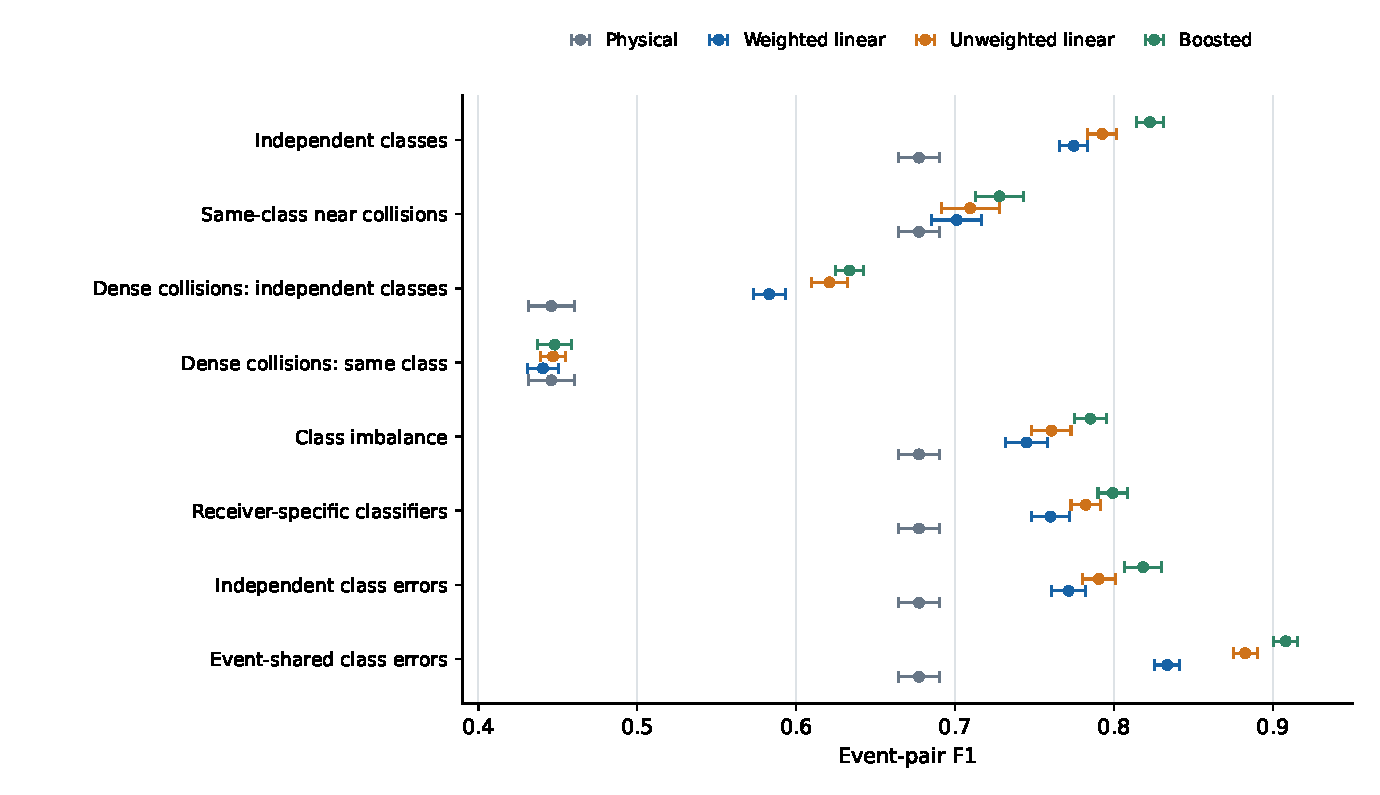
\includegraphics[width=\linewidth]{figures/deep_semantic_stress.pdf}
\caption{Semantic interventions on independent descriptor scenes. All class maps are supplied. Error bars use replication-level intervals. The dense same-class condition shows no clear semantic advantage in this experiment. Shared within-event errors preserve compatibility despite wrong class predictions.}\label{fig:deep_semantic}
\end{figure}

Every semantic-only intervention preserves the physical report arrays. Physical-only F1 is consequently identical across those paired conditions. The dense pair has its own physical reference. Verification reproduces 800 nominal and dense source scenes exactly. Independent checks also compare 576 physical fields with the original generator across 48 condition--seed cases. Replacing event and clutter labels leaves inference batches and checked predictions unchanged. All 12,800 outputs meet the receiver and gate constraints. The saved files include per-scene TP, FP, FN, all partition metrics, replication means, paired differences, and predictions. Pooled micro F1 is stored separately from scene-macro F1.
\FloatBarrier

\subsection{Public timestamp tails and a metadata clock comparator}
The script is \texttt{code/deep\_loed\_audit.py}. It reads the unchanged publisher sample and retained observation IDs. A tail diagnostic uses an absolute corrected time difference above 10 ms. It changes no inclusion decision or reference label. Table~\ref{tab:deep_loed_tail} shows all six captures, including April's lack of a cross-gateway reference pair.

\begin{table}[!htb]\caption{Corrected reference-pair time differences. Tail means an absolute difference above 10 ms. The last column counts tails with different reported channels. The 2019 receiver pair has no supported clock correction. Every central 2020 pair has matching channels. All records remain in the evaluation.}\label{tab:deep_loed_tail}
\scriptsize\setlength{\tabcolsep}{3pt}\begin{tabularx}{\linewidth}{@{}Yrrrrr@{}}\toprule
Capture & Reference pairs & Median ($\mu$s) & $Q_{0.99}$ (ms) & $>10$ ms & Channel mismatch in tail \\\midrule
2019-03-03 & 1 & 66771.6 & 66.772 & 1 & 0 \\
2019-04-02 & 0 & -- & -- & -- & -- \\
2020-05-02 & 256 & 4.0 & 2100.826 & 5 & 5 \\
2020-07-03 & 434 & 5.0 & 3.025 & 4 & 4 \\
2020-08-03 & 903 & 16.0 & 0.146 & 0 & 0 \\
2020-09-02 & 514 & 15.0 & 2.122 & 2 & 2 \\
\bottomrule\end{tabularx}
\end{table}

The eleven 2020 tail pairs have matching full PHY payloads, device addresses, frame counters, and spreading factors, but different channel frequencies. Each complete payload occurs in exactly two raw rows at two gateways, both with valid CRC, so they pass the existing one-record-per-gateway rule and five-second raw-span exclusion. The raw sample contains only one time field and cannot distinguish repeated transmissions from metadata errors. This reference ambiguity remains unresolved.

July's 434 sorted residuals have median $5\,\mu$s and 95th percentile $22\,\mu$s. Its 0.99 quantile has zero-based rank 428.67. Linear interpolation uses 2.120 and 3.471 ms. Its 0.999 quantile has rank 432.567 and uses 2.136977 and 4.201604 s. This gives 3.307620509 s. The endpoint record permits direct reproduction of the jump. Supported-pair raw signed medians from May through September are 0.999985, 0.999986, 1.000001, and 1.000000 s. These central shifts do not explain the seconds-long tails.

The alternative clock estimator receives only training day, gateway, timestamp, channel, and spreading factor. It forms matching-channel and matching-SF candidate lags in $[-5,5]$ s. Histogram bins are 1 ms wide. The strongest bin defines a refinement neighborhood of $\pm5$ ms. At least ten entries are required in the peak bin. At least twenty are required in the refinement. The peak must be at least five times the larger of one and the 99th percentile of all bin counts. It must also be at least twice the larger of one and the strongest bin beyond 10 ms from its center. Supported pair lags enter the same count-weighted least-squares clock system as the reference method. Unsupported corrections remain zero.

The 2020 pair supplies 343 metadata candidates. Its peak bin has 242 entries. The refinement has 251. The median lag is 0.999985 s. The 2019 pair supplies 38 candidates and peak count one. It remains unsupported. The largest difference between the two fitted receiver-correction vectors is $2.22\times10^{-16}$ s. Synthetic estimator checks recover a known 0.37 s shift with correct sign. Two equally strong separated modes are rejected. These checks do not represent new measured recordings.

\begin{table}[!htb]\caption{Clock fitting with unchanged public test reports. Reference support counts training payload matches. Metadata support counts lags in the fixed refinement neighborhood. Scorer fitting, gate calibration, and population selection remain reference-assisted. Both clock fits give identical test partitions.}\label{tab:deep_loed_clock}
\small\setlength{\tabcolsep}{3pt}\begin{tabularx}{\linewidth}{@{}Yrrrrr@{}}\toprule
Clock fit & Training support & Lag (s) & TP / FP / FN & $G$ (ms) & Packet F1 \\\midrule
Payload-reference median & 256 & 0.999985 & 1411 / 1 / 6 & 3.025 & 0.9975 \\
Metadata lag mode & 251 & 0.999985 & 1411 / 1 / 6 & 3.025 & 0.9975 \\
\bottomrule\end{tabularx}
\end{table}

The estimator settings are fixed for this secondary comparison without selection on test F1. Because the public captures had already been inspected, the comparison is not an independent prospective deployment test. The 2019-only training setting changes gateway coverage and positive support together with date, so its zero F1 cannot isolate temporal drift. All raw tail rows, quantile endpoints, support counts, fitted offsets, and test predictions are retained.
\FloatBarrier

\subsection{Fixed-registry report-path latency}
The script \texttt{code/deep\_runtime.py} uses ten fresh instances at each of $N=40,80,120$. The sizes use separate scenes. Their generator event counts are 18, 30, and 43. Selection uses report count alone. A random subset supplies the requested number of reports. The frozen weighted linear scorer is used throughout. Within each instance, every decoder receives the same reports and score model.

The timed path starts with native feature construction. It includes frozen scoring and event decoding. Descriptor generation, file I/O, waveform processing, and offline map fitting are excluded. Greedy and restart paths use the median of three contiguous measurements per instance. MILP uses one solve per instance. Initialization occurs outside the intervals. Reference metrics and feasibility checks also occur outside the intervals. The full triangle MILP includes sparse construction and label reconstruction in its reported path time. Preallocated sparse arrays reduce Python object overhead. The mathematical formulation is unchanged.

\begin{table}[!htb]\caption{Fresh fixed-registry report-path measurements. Each size uses ten independently seeded scenes. Median and maximum refer to instance-level path times. F1 averages ten scene values. The one-second cap applies to the solver only. Model construction is included in the reported path. Every MILP result is proven optimal.}\label{tab:deep_runtime}
\small\setlength{\tabcolsep}{3pt}\begin{tabularx}{\linewidth}{@{}rYrrrrr@{}}\toprule
$N$ & Decoder & Median (ms) & Maximum (ms) & Event F1 & Proven / 10 & Timeouts \\\midrule
40 & Greedy & 0.64 & 0.69 & 0.8068 & -- & -- \\
40 & Restart & 2.52 & 2.69 & 0.7841 & -- & -- \\
40 & MILP & 34.56 & 37.53 & 0.7781 & 10 & 0 \\
80 & Greedy & 1.80 & 1.92 & 0.7673 & -- & -- \\
80 & Restart & 8.03 & 8.50 & 0.7653 & -- & -- \\
80 & MILP & 284.37 & 335.45 & 0.7705 & 10 & 0 \\
120 & Greedy & 3.63 & 3.85 & 0.7830 & -- & -- \\
120 & Restart & 17.73 & 18.10 & 0.7841 & -- & -- \\
120 & MILP & 956.65 & 1014.16 & 0.7836 & 10 & 0 \\
\bottomrule\end{tabularx}
\end{table}

All 30 solves prove optimality without reaching the requested solver limit. The largest 120-report path takes 1014.16 ms because construction precedes optimization. These times describe the tested full formulation and environment, rather than a bound on all MILP implementations. At 40 reports, greedy mean event F1 is 0.8068 and MILP F1 is 0.7781. More objective search need not improve event accuracy. Different scenes and event densities also prevent a size-only interpretation of F1 changes across rows.

One separate Windows process measures a 120-report solve's memory. Its resident working set is 146,747,392 bytes before the solve. Peak working set reaches 650,665,984 bytes, or about 620.5 MiB. This includes Python, numerical libraries, sparse construction, and HiGHS. Initial sparse arrays occupy 40,440,960 bytes. The process peak is a measured example, not a memory upper bound. The case has 7140 variables and 842,520 triangle inequalities.

\subsection{Files and commands for the independent validation}
All new scientific outputs are under \texttt{results/deep\_revision/}. Mapping outputs are in \texttt{mapping}. Semantic interventions are in \texttt{semantic\_stress}. The remaining folders are \texttt{loed}, \texttt{runtime}, and \texttt{models}. Each experiment records its protocol, seeds or input identifiers, parameters, and checks. The dependency lock remains \texttt{requirements-review-lock.txt}. The following commands run from this project folder:
\begin{verbatim}
python code/deep_revision.py --task all
python code/deep_revision.py --task verify
\end{verbatim}
The first command executes the added experiments sequentially. The second checks retained outputs and invariants. Old scientific results remain in their original subdirectories. All comparisons use scene- or replication-level summaries as stated. Repeated solver or scorer evaluations do not create additional independent scenes.

\end{document}
